\documentclass[11pt,a4paper]{article}

% --- Geometry & Layout ---
\usepackage[margin=1in]{geometry}
\usepackage{parskip}
\usepackage[T1]{fontenc}
\usepackage[utf8]{inputenc}

% --- Section Formatting ---
\usepackage{titlesec}
\usepackage{tocloft}

% --- Colors & Boxes ---
\usepackage[dvipsnames,svgnames]{xcolor}
\usepackage[most]{tcolorbox}

% --- Lists & Tables ---
\usepackage{enumitem}
\usepackage{booktabs}
\usepackage{longtable}
\usepackage{tabularx}

% --- Code Listings ---
\usepackage{listings}

% --- Graphics ---
\usepackage{tikz}
\usetikzlibrary{arrows.meta,positioning,shapes.geometric,fit,calc,backgrounds}

% --- Hyperlinks ---
\usepackage[colorlinks=true,linkcolor=NavyBlue,urlcolor=RoyalBlue,citecolor=NavyBlue]{hyperref}

% --- Headers & Footers ---
\usepackage{fancyhdr}
\pagestyle{fancy}
\fancyhf{}
\fancyhead[L]{\small\textsc{Levshell Specification}}
\fancyhead[R]{\small\textsc{v0.2 --- Draft}}
\fancyfoot[C]{\thepage}
\renewcommand{\headrulewidth}{0.4pt}

% ===========================================================================
% Custom Colors
% ===========================================================================
\definecolor{levblue}{HTML}{7AA2F7}
\definecolor{levpurple}{HTML}{BB9AF7}
\definecolor{levgreen}{HTML}{9ECE6A}
\definecolor{levorange}{HTML}{E0AF68}
\definecolor{levred}{HTML}{F7768E}
\definecolor{levbg}{HTML}{1A1B26}
\definecolor{levfg}{HTML}{C0CAF5}
\definecolor{codebg}{HTML}{F0F0F4}

% ===========================================================================
% Custom Environments
% ===========================================================================
\newtcolorbox{designbox}[1][]{
  colback=levblue!5,
  colframe=levblue!60!black,
  fonttitle=\bfseries,
  title={#1},
  arc=2pt,
  boxrule=0.5pt,
  left=6pt, right=6pt, top=4pt, bottom=4pt,
}

\newtcolorbox{principlebox}[1][]{
  colback=levpurple!5,
  colframe=levpurple!60!black,
  fonttitle=\bfseries,
  title={#1},
  arc=2pt,
  boxrule=0.5pt,
  left=6pt, right=6pt, top=4pt, bottom=4pt,
}

\newtcolorbox{notebox}[1][]{
  colback=levorange!5,
  colframe=levorange!60!black,
  fonttitle=\bfseries,
  title={#1},
  arc=2pt,
  boxrule=0.5pt,
  left=6pt, right=6pt, top=4pt, bottom=4pt,
}

% --- Code Listing Style ---
\lstset{
  backgroundcolor=\color{codebg},
  basicstyle=\ttfamily\small,
  breaklines=true,
  frame=single,
  rulecolor=\color{gray!40},
  keywordstyle=\color{NavyBlue}\bfseries,
  commentstyle=\color{OliveGreen}\itshape,
  stringstyle=\color{BrickRed},
  showstringspaces=false,
  tabsize=2,
  xleftmargin=4pt,
  xrightmargin=4pt,
  aboveskip=8pt,
  belowskip=8pt,
}

% --- Title Formatting ---
\titleformat{\section}{\Large\bfseries\color{NavyBlue}}{\thesection}{1em}{}[\vspace{-4pt}\textcolor{levblue}{\rule{\textwidth}{0.5pt}}]
\titleformat{\subsection}{\large\bfseries\color{NavyBlue!80}}{\thesubsection}{1em}{}
\titleformat{\subsubsection}{\normalsize\bfseries\color{NavyBlue!60}}{\thesubsubsection}{1em}{}

% --- TOC Formatting ---
\renewcommand{\cftsecleader}{\cftdotfill{\cftdotsep}}

% ===========================================================================
% Document Begin
% ===========================================================================
\begin{document}

% --- Title Page ---
\begin{titlepage}
\centering
\vspace*{2cm}

{\Huge\bfseries\color{NavyBlue} Levshell\par}
\vspace{0.5cm}
{\Large\color{NavyBlue!70} A Context-Aware Research Environment\\for the Sway Window Manager\par}

\vspace{1cm}
\textcolor{levblue}{\rule{0.6\textwidth}{1pt}}

\vspace{1.5cm}
{\large\textsc{Specification Document}\par}
\vspace{0.3cm}
{\normalsize Version 0.2 --- Draft\par}
\vspace{0.3cm}
{\normalsize\today\par}

\vspace{3cm}

\begin{principlebox}[Guiding Principle]
A blissful mix of elegance and absolute productivity. A shell that gets out of your way when needed, but is there almost like an omnipotent catalyst to help you through difficult patches of work.
\end{principlebox}

\vspace{2cm}

{\small\textit{Built with QuickShell (QML) for rendering and a Rust daemon for logic.\\A hybrid architecture: unified data model with incremental tool replacement.\\Designed for Wayland/Sway. Engineered for researchers and students.}\par}

\vfill
\end{titlepage}

% --- Table of Contents ---
\newpage
\tableofcontents
\newpage

% ===========================================================================
% PART I: VISION & FEATURES
% ===========================================================================

\section{Introduction}
\label{sec:intro}

Levshell is a context-aware research environment for the Sway window manager on Wayland-based Linux systems. Its purpose is to catalyze productivity, particularly for students and researchers in computer science and artificial intelligence. Unlike conventional desktop bars and panels, which display a fixed set of widgets regardless of user context, Levshell dynamically adapts its interface to the user's current task, open projects, and cognitive state.

Levshell is more than a shell. It is designed as an \textbf{integrated research environment}: a suite of tools---knowledge base, reference manager, spaced repetition system, calendar, task manager---that share a unified data model and are orchestrated by a context-aware shell. The shell is the visible surface; the unified data model is the foundation.

\subsection{Hybrid Architecture Strategy}

Levshell adopts a \textbf{hybrid approach} to reach the goal of a fully integrated suite while remaining usable at every stage of development:

\begin{enumerate}[leftmargin=1.5em, itemsep=4pt]
  \item \textbf{Define the unified data model first.} Projects, notes, references, flashcards, events, tasks, and experiments are first-class entities in a shared schema (see Section~\ref{sec:data-model}). All shell logic---the context engine, ideation nudges, cross-tool queries---operates on this model, never on tool-specific data formats.

  \item \textbf{Initially populate the model by syncing from existing tools.} Provider implementations for Zotero, Obsidian, Anki, and others act as \emph{import/sync adapters} that translate external data into the unified model. The shell and daemon operate entirely on the unified model, not on the tools directly.

  \item \textbf{Incrementally replace external tools with native components.} Over time, individual sync adapters are replaced by native Levshell components---a built-in knowledge base, a built-in SRS, a built-in reference manager---that write directly to the unified model. Each replacement is independent, and at every stage the system is fully functional.
\end{enumerate}

This approach captures the core advantage of a full suite (unified data, deep cross-tool intelligence, total control over the user experience) while allowing the system to ship on top of existing tools immediately. The migration from ``shell that syncs with Zotero'' to ``shell with built-in reference manager'' is gradual, not a big bang.

\begin{designbox}[Architectural Invariant]
All shell logic depends on the unified data model, never on a specific tool or provider. Whether a reference entry was synced from Zotero or created natively, it is the same entity in the same schema. This invariant ensures that every native component replacement is transparent to the rest of the system.
\end{designbox}

\subsection{System Components}

The system is built on three foundational components:

\begin{enumerate}[leftmargin=1.5em, itemsep=3pt]
  \item \textbf{QuickShell} (QML): The rendering layer. Draws the bar, handles input, displays what the daemon tells it to.
  \item \textbf{levshell-daemon} (Rust): The brain. Owns the unified data model, event bus, context engine, module system, and all integration logic.
  \item \textbf{Unified Data Store}: A structured database (embedded, e.g., SQLite or sled) that holds the canonical representation of all research entities. Both sync adapters and native components read and write to this store.
\end{enumerate}

\subsection{Design Principles}

\begin{principlebox}[Core Design Principles]
\begin{enumerate}[leftmargin=1.5em, itemsep=3pt]
  \item \textbf{Unified model is the source of truth.} All shell logic operates on the shared data model. External tools are data sources, never direct dependencies of the shell's behavior.
  \item \textbf{Context-awareness over configuration.} The shell should infer what the user needs from observable signals (active window, workspace, time, running processes) and adapt automatically, with manual overrides always available.
  \item \textbf{Quiet until important.} Widgets, notifications, and metrics should remain invisible during normal operation and surface only when their information becomes actionable.
  \item \textbf{Elegance is not optional.} Every interaction, animation, and visual element must be deliberate. Visual noise is a productivity cost.
  \item \textbf{Modularity at every layer.} Every feature is a module. Adding, removing, or reconfiguring a feature should never require touching the core system.
  \item \textbf{The bar is the primary interface.} The top bar is not a passive display---it is the user's command center, research dashboard, and ambient awareness layer.
  \item \textbf{Researcher-native.} Features are designed around the workflows of academic researchers: reading papers, writing \LaTeX{}, running experiments on remote clusters, managing citations, retaining knowledge.
  \item \textbf{Incremental migration.} The system must be fully functional at every stage---from ``sync adapter for every tool'' to ``fully native suite.'' No big-bang migration.
\end{enumerate}
\end{principlebox}


% ===========================================================================
\section{Feature Specification}
\label{sec:features}

This section exhaustively enumerates the features planned for Levshell. Features are categorized by domain. Each feature may be implemented as a core component, a default module, or an optional extension.

% ---------------------------------------------------------------------------
\subsection{Top Bar Layout \& Global UX}
\label{sec:features-bar}

\subsubsection{Global Menu Bar}
The active application's menu hierarchy (File, Edit, View, etc.) renders in the top bar rather than inside the application window, following the macOS convention. This reclaims vertical space in every application and provides a single, predictable location for menu actions. For GTK and Qt applications that export menus over D-Bus (via the \texttt{com.canonical.AppMenu.Registrar} interface), menus are displayed natively. For applications without menu export, a fallback display shows the application name and focused window title.

\subsubsection{Unified Command Palette}
A single keystroke summons a search-driven overlay inspired by Spotlight, Raycast, and Rofi, but native to the shell. The command palette serves as the universal entry point for: application launching, shell command execution, file search, workspace switching, recent document access, calculator and unit/currency conversion, Unicode/emoji lookup, and every Levshell subsystem (module settings, project search, Anki card creation, Zotero lookup, etc.). All searchable surfaces in the shell register themselves with the command palette as search providers.

\subsubsection{Breadcrumb Workspace Indicator}
Instead of numbered boxes, the workspace indicator displays a breadcrumb path: workspace name, separator, focused window title---elegantly truncated. Each segment is interactive: clicking navigates or renames; drag-and-drop moves windows between workspaces.

\subsubsection{Morphing Bar Density}
The bar operates in three density modes:
\begin{itemize}[leftmargin=1.5em, itemsep=2pt]
  \item \textbf{Full}: All widgets visible with labels.
  \item \textbf{Compact}: Icons only; hover to expand individual widgets.
  \item \textbf{Hidden}: Bar is invisible; auto-shows on pointer push to screen edge or keybind.
\end{itemize}
Transitions are animated. Density can be set per-workspace or globally, and overridden with a keybind.

\subsubsection{Clock \& Calendar Hub}
The center clock doubles as a dropdown hub displaying: a mini calendar view, upcoming events (synced from CalDAV, Google Calendar, or local ICS files), a world-clock row for collaborators in other time zones, and a countdown timer for the next upcoming event that appears in the bar 15 minutes before start.

\subsubsection{Notification Center}
A single aggregation point for all desktop notifications (via the freedesktop notification specification). The dropdown groups notifications by application, supports inline reply for chat applications, and includes a focus mode toggle that silences all notifications except those from starred senders. Missed notifications persist and can be snoozed or pinned.

\subsubsection{Quick-Settings Flyout}
A single-click panel (analogous to macOS Control Center) providing: volume and brightness sliders, night-light warmth control, and toggles for Wi-Fi, Bluetooth, Do Not Disturb, screen recording, and VPN. Each tile can expand for detail (e.g., Wi-Fi shows available networks, Bluetooth shows paired devices with battery levels).


% ---------------------------------------------------------------------------
\subsection{Productivity \& Focus}
\label{sec:features-productivity}

\subsubsection{Pomodoro / Session Timer}
A compact pill in the bar showing elapsed focus time. Configurable work/break intervals with auto-logging of sessions per workspace. Break reminders respect Do Not Disturb state. Optionally dims or tints the screen during breaks.

\subsubsection{Daily Planner Glance}
A collapsible widget displaying today's agenda as a vertical timeline, sourced from calendar sync. Tasks from Todoist, Taskwarrior, or plain Markdown files can be interleaved. Tasks can be completed inline from the widget.

\subsubsection{Scratch Pad / Quick Capture}
A keybind opens a small floating text input anchored to the bar. Typed content is appended to a configurable capture file (Markdown, Org-mode, or Zettelkasten inbox). Supports image pasting, which saves images to an assets directory and inserts a link automatically.

\subsubsection{Reading List Queue}
A dropzone in the bar accepts dragged URLs or PDFs, adding them to a reading list. The widget displays an unread count and allows cycling through queued items.

\subsubsection{Global Word/Character Count}
When a text editor or word processor is focused, a subtle counter displays live word count, character count, and estimated page count.

\subsubsection{Session Journal}
On demand or at end-of-day, Levshell auto-generates a summary of the session: applications used, files touched, workspaces visited, focus time logged. Exportable as Markdown.


% ---------------------------------------------------------------------------
\subsection{System Telemetry \& Resource Awareness}
\label{sec:features-telemetry}

\subsubsection{Adaptive System Telemetry}
CPU, RAM, temperature, disk I/O, and network throughput displayed as compact sparkline graphs. Widgets are configured to appear only when values exceed configurable thresholds (e.g., CPU $>$ 60\%), implementing the ``quiet until important'' principle.

\subsubsection{Battery \& Power Profile}
Battery icon with estimated time remaining. Click to switch between power profiles (power-saver, balanced, performance) via \texttt{power-profiles-daemon} or TLP. Displays current wattage draw when hardware supports it.

\subsubsection{Network Quality Indicator}
Beyond connection status: displays latency to a configurable endpoint (e.g., university VPN gateway), throughput rates, and a color-coded quality dot (green/yellow/red).

\subsubsection{Disk Space Warning}
Invisible until free space on any mounted volume drops below a configurable threshold, at which point it surfaces with a cleanup shortcut.

\subsubsection{Process Sniper}
Long-press or right-click the CPU graph to see the top 5 resource-consuming processes. One click sends \texttt{SIGTERM}; shift-click sends \texttt{SIGKILL}.


% ---------------------------------------------------------------------------
\subsection{Workspaces \& Window Management}
\label{sec:features-workspaces}

\subsubsection{Named \& Persistent Workspaces}
Workspaces have human-readable names and optionally persist their window layout across reboots---which applications, which positions, which monitors.

\subsubsection{Workspace Thumbnails}
Hovering over a workspace indicator shows a live mini-preview of its contents, similar to macOS Mission Control.

\subsubsection{Workspace Templates}
Pre-defined layout templates that can be instantiated: e.g., ``Research'' opens a browser on the left half, PDF reader top-right, notes application bottom-right, all pre-tiled.

\subsubsection{Window Grouping / Tabs}
Multiple windows can be grouped into a tabbed container within a workspace. The tab bar is styled by Levshell and can reside in the top bar area or float above the group.

\subsubsection{Scratchpad Manager}
A bar widget displaying the number of windows in Sway's scratchpad with a dropdown list for peeking and cycling through them.

\subsubsection{Picture-in-Picture}
Pin any window as a floating, always-on-top, resizable, opacity-adjustable thumbnail.

\subsubsection{Workspace Activity Indicator}
A subtle visual cue (glow or dot) on workspace labels that have had recent unacknowledged activity.


% ---------------------------------------------------------------------------
\subsection{File \& Clipboard Management}
\label{sec:features-clipboard}

\subsubsection{Clipboard History}
A ring buffer of the last $N$ clipboard entries (text, images, files). Searchable from the command palette or a dedicated dropdown. Supports pinning frequently-used snippets.

\subsubsection{Clipboard Transformations}
Paste-as actions: plain text, URL auto-linked, Markdown-to-HTML, formatted code block, or output of a user-defined transformation script.

\subsubsection{Drag-and-Drop Shelf}
A tray area in the bar for parking files or text snippets mid-workflow. Drag content to the shelf, switch workspaces, drag it out at the destination.

\subsubsection{Recent Files}
A dropdown of recently opened/modified files, grouped by application or workspace.

\subsubsection{Quick File Preview}
Hovering over a file in the shelf or recent-files list shows a thumbnail or text preview.


% ---------------------------------------------------------------------------
\subsection{Search \& Knowledge}
\label{sec:features-search}

\subsubsection{Unified Desktop Search}
Indexes local files (content and metadata), browser bookmarks, application entries, man pages, and notes. Results appear in the command palette with categorized sections. Custom search providers can be registered (Arch Wiki, arXiv, Stack Overflow, etc.).

\subsubsection{Dictionary / Thesaurus Lookup}
Highlight a word, invoke a keybind, and receive a popover with definition, synonyms, and etymology.

\subsubsection{Quick Translation}
Same interaction flow as dictionary lookup but sends the selection to a translation engine (DeepL, LibreTranslate, or a local model).

\subsubsection{Formula Reference}
A searchable sheet of mathematical formulas, Greek letters, and \LaTeX{} symbol names. Selecting an entry copies the \LaTeX{} command, Unicode character, or both.

\subsubsection{Snippet / Template Library}
A searchable repository of text templates---email boilerplate, \LaTeX{} preambles, code snippets, regex patterns---insertable into the focused application.


% ---------------------------------------------------------------------------
\subsection{Communication \& Social}
\label{sec:features-comms}

\subsubsection{Unified Inbox Indicator}
A single icon with a badge count aggregating unreads from email (IMAP/Notmuch), chat (Matrix, Slack, Discord), and calendar reminders. Clicking expands a grouped list.

\subsubsection{Quick Reply}
For supported protocols, reply inline from the notification dropdown.

\subsubsection{Meeting Join Button}
When a calendar event with a video-call link is approaching, a ``Join'' button appears in the bar.

\subsubsection{Presence / Status Broadcast}
Set status (``focusing,'' ``in class,'' ``available'') from the bar and broadcast to configured services simultaneously.


% ---------------------------------------------------------------------------
\subsection{Media \& Ambient}
\label{sec:features-media}

\subsubsection{MPRIS Media Controls}
Play/pause, track navigation, progress bar, and album art for the active MPRIS-compatible media player. Supports multiple simultaneous sources with a switcher.

\subsubsection{Now-Playing Display}
Current track title as scrolling text or tooltip. Optional scrobbling to Last.fm or ListenBrainz.

\subsubsection{Per-Application Volume Mixer}
Per-application volume control via PipeWire, accessible from a flyout.

\subsubsection{Ambient Soundscapes}
Built-in white noise, rain, or lo-fi generator (or controller for an external one) accessible from the bar.

\subsubsection{Night-Light / Color Temperature}
A warmth slider or automatic scheduling. Optional ``paper'' mode that shifts the color profile for extended reading.


% ---------------------------------------------------------------------------
\subsection{Academic \& Research}
\label{sec:features-academic}

\subsubsection{Open Project Registry}
\label{sec:features-projects}
A first-class data model for ``open projects.'' Each project has a name, status (active, simmering, blocked, writing-up, complete), description, a list of open questions, associated tags, and links to external systems: Obsidian vault paths, Zotero collections, Git repositories, Anki tags, SSH hosts, BibTeX files, deadlines, and collaborators.

Projects are the fundamental unit of research context in Levshell. Other modules query the project registry to correlate their data with the user's active research threads.

\subsubsection{Stochastic Ideation Nudges}
At semi-random intervals (Poisson-distributed around a configurable mean, e.g., $\lambda = 45$ minutes), a non-modal notification surfaces a prompt tied to an open project. Prompts are drawn from: the project's open questions, recent Obsidian highlights, or detected cross-project connections. Nudges are suppressed during focus sessions and queued for delivery during transitions (workspace switch, screen unlock, break period).

\subsubsection{Cross-Project Connection Surfacing}
When a new Obsidian note or Zotero entry is added, the system checks for tag, keyword, and author overlaps with other open projects. Connections are surfaced as nudge-style notifications.

\subsubsection{Project Pulse Indicator}
A compact bar widget showing which projects have had activity today and which have been dormant beyond a configurable threshold. Clicking expands a dashboard: last touched, hours logged, upcoming deadlines, open questions, recent notes.

\subsubsection{Blocked-Project Escalation}
If a project is marked ``blocked'' or has been untouched for a configurable period, ideation nudge frequency increases and shifts to unblocking prompts: smallest concrete next step, or the user's own recorded blocker note.

\subsubsection{Anki Integration}
\label{sec:features-anki}
\begin{itemize}[leftmargin=1.5em, itemsep=2pt]
  \item \textbf{Review due counter}: Persistent badge in the bar showing cards due. Color-coded by urgency. Click to open Anki or a minimal review overlay via AnkiConnect.
  \item \textbf{Inline card creation}: Highlight text anywhere, invoke keybind, populate a card creation popup. Auto-tags with the current workspace or project.
  \item \textbf{Context-triggered review}: When switching to a workspace associated with a topic that has due Anki cards, suggest reviewing those cards first.
  \item \textbf{Spaced repetition for open questions}: Open project questions are surfaced on a spaced repetition schedule, blurring the line between flashcards and the ideation engine.
  \item \textbf{Retention heatmap}: Dashboard view of retention rates by deck/tag over time.
\end{itemize}

\subsubsection{Obsidian / Knowledge Base Integration}
\label{sec:features-obsidian}
\begin{itemize}[leftmargin=1.5em, itemsep=2pt]
  \item \textbf{Graph-aware shell}: Indexes the vault's link structure. Knows hubs, orphans, recent notes, and dense clusters.
  \item \textbf{Orphan note surfacing}: Periodically identifies notes with no backlinks and prompts the user to link or archive them.
  \item \textbf{Daily note integration}: Pulls today's tasks and open loops from Obsidian daily notes into a bar widget. Inline completion syncs back to the Markdown file.
  \item \textbf{Vault search}: Full-text search across the vault from the command palette.
  \item \textbf{Context recall}: When returning to a workspace after absence, shows the last notes and files that were open, reducing re-entry cost.
  \item \textbf{Inbox monitor}: Badge for unprocessed fleeting notes with nudges to process them.
  \item \textbf{Note velocity}: Tracks notes created/modified per day/week, broken down by project.
\end{itemize}

\subsubsection{Zotero \& Literature Management}
\label{sec:features-zotero}
\begin{itemize}[leftmargin=1.5em, itemsep=2pt]
  \item \textbf{Library stats widget}: Total papers, unread count, recently added items.
  \item \textbf{Related work radar}: When a paper is added, checks its references and authors against the existing library for overlaps.
  \item \textbf{Reading progress}: Tracks current page in the active PDF reader per paper.
  \item \textbf{Annotation extractor}: Pulls highlights from PDFs and pushes them to Obsidian as literature note scaffolds.
  \item \textbf{Citation graph explorer}: Mini citation graph via Semantic Scholar or OpenAlex data.
  \item \textbf{Citation quick-search}: Bar widget to search BibTeX/Zotero and copy formatted citekeys.
  \item \textbf{Conference deadline integration}: Pulls deadlines from curated sources; escalates relevant project nudges as deadlines approach.
  \item \textbf{BibTeX health checker}: Periodic linting of \texttt{.bib} files for missing fields, duplicates, and unreferenced entries.
\end{itemize}

\subsubsection{arXiv / Semantic Scholar Watcher}
Configure keywords or followed authors. A badge appears when new matching papers are found. Click to see titles and abstracts; click through to open the PDF.

\subsubsection{\LaTeX{} Compilation Status}
When a \LaTeX{} build is running, a progress/status indicator appears in the bar (compiling $\to$ success/error). Click to view the log on error.

\subsubsection{Lecture / Meeting Recorder}
One-click screen and audio recording from the bar with automatic timestamping. Optional transcription via Whisper with transcript linked to notes.

\subsubsection{Deadline Tracker}
Upcoming deadlines from calendars, task managers, or plain text files. Color-coded by urgency.


% ---------------------------------------------------------------------------
\subsection{SSH \& Remote Systems}
\label{sec:features-ssh}

\subsubsection{SSH Connection Dashboard}
A bar widget showing all active SSH sessions: named hosts, connection duration, associated workspace, and a color-coded latency indicator (green/yellow/red). Immediate notification with one-click reconnect on connection drop.

\subsubsection{Named Host Profiles}
A host registry with human-readable names (``Lab GPU Cluster,'' ``University HPC''), associated project, and notes. These names replace raw hostnames throughout the shell.

\subsubsection{Remote Job Monitor}
For long-running remote jobs (training runs, benchmarks, compilations), the daemon polls status via log tailing over SSH, SLURM/PBS queue queries, or status files. A bar widget displays job name, host, progress, key metrics (e.g., epoch, loss), and ETA.

\subsubsection{GPU Utilization Dashboard}
Polls \texttt{nvidia-smi} or equivalent on remote hosts. Displays GPU utilization, memory usage, temperature, and running processes.

\subsubsection{Remote Filesystem Bookmarks}
Quick-access bookmarks to remote directories via SFTP/SSHFS. Click to mount; click again to open in a file manager or terminal.

\subsubsection{SSH Tunnel Manager}
Displays active port forwards and tunnels. Create new tunnels from the bar (e.g., forward local 8888 to remote 8888 for Jupyter). Visual indicator for active tunnels.

\subsubsection{Experiment Tracker Integration}
Surfaces run summaries from Weights \& Biases, MLflow, or custom logging: which experiments ran, key metrics, running status.

\subsubsection{Cluster Queue Status}
Polls SLURM/PBS queues. Displays: system-wide queue depth, user's queued/running jobs, priority/fairshare, and estimated start time for pending jobs.

\subsubsection{SSH Session Logging}
Optional timestamped logging of SSH sessions (connection time, host, initial command) for correlation with the local session journal.


% ---------------------------------------------------------------------------
\subsection{Code \& Development Awareness}
\label{sec:features-code}

\subsubsection{Build / CI Status}
Polls GitHub Actions, GitLab CI, or local build systems. Displays red/green status per project. Click to view failure logs.

\subsubsection{Git Status per Project}
For each open project with a Git repository: current branch, uncommitted changes count, unpushed commits count, and divergence from upstream.

\subsubsection{Compiler Error Flash}
When a build fails in a terminal, captures the first error message and displays a persistent notification with file and line reference. Click to open the editor at that location.

\subsubsection{Dependency Vulnerability Alerts}
Periodic lightweight audits (\texttt{cargo audit}, \texttt{pip-audit}, \texttt{npm audit}) with badge notification on findings.

\subsubsection{Docker / Container Status}
Displays running containers, their exposed ports, and resource usage. One-click stop/restart.

\subsubsection{Lab Notebook}
Structured experiment log: hypothesis, setup (git commit, config, hardware), results, notes. Levshell auto-populates fields (commit hash, hostname, timestamp) on new entries.


% ---------------------------------------------------------------------------
\subsection{Deep Focus \& Cognitive Support}
\label{sec:features-focus}

\subsubsection{Warmup Mode}
On session start (first unlock of the day or after long idle), offers a gentle ramp-up: review agenda, check Anki dues, glance at project statuses, then transition into focused work.

\subsubsection{Context Save / Restore}
A keybind snapshots the current state---open windows, terminal scrollback, editor positions, browser tabs, audio---and names it. Restoring returns to the exact state. This is the unit of context-switching.

\subsubsection{Interruption Cost Awareness}
When returning to a focused workspace after a context switch, a subtle timer indicates time since departure---not punitive, just awareness of re-entry cost.

\subsubsection{Literature Review Mode}
A context profile for deep reading: Zotero search prominent, annotation shortcuts visible, Anki card creation keybind active, media and notifications suppressed. Auto-triggered when a PDF reader is focused for a sustained period.

\subsubsection{Writing Mode}
When \LaTeX{} or a Markdown editor is focused: word count visible, citation search prominent, build status shown, distraction-free bar option available.

\subsubsection{Rubber Duck Debugger}
A bar button opening a minimal chat interface (connected to a local LLM or structured prompt template) for articulating and debugging stuck points.


% ---------------------------------------------------------------------------
\subsection{Data \& Experiment Pipeline}
\label{sec:features-data}

\subsubsection{Dataset Registry}
A catalog of frequently-used datasets with metadata: location (local, remote, S3), size, last accessed, associated project.

\subsubsection{Storage Quota Monitor}
Monitors university storage, NFS mounts, and cloud buckets. Warns before quota limits are hit.

\subsubsection{Reproducibility Snapshot}
A keybind captures the current experimental environment: git hash, dependency freeze, hardware specs, config files. Written to a structured log.

\subsubsection{Paper-to-Code Linker}
Maintains mappings between Zotero entries and code repositories (both reference implementations and personal reimplementations).


% ---------------------------------------------------------------------------
\subsection{Health \& Wellbeing}
\label{sec:features-health}

Includes: eye break reminders (20-20-20 rule), posture/stretch reminders, daily screen time tracking (broken down by app/workspace), and an optional hydration tracker. All reminders are non-intrusive and respect focus sessions.


% ---------------------------------------------------------------------------
\subsection{Security \& Privacy}
\label{sec:features-security}

Includes: VPN status indicator with one-click connect, password manager integration (KeePassXC, Bitwarden CLI, \texttt{pass}) for OTP/password access from the bar, a visible screen lock button, and an always-visible camera/microphone activity indicator.


% ---------------------------------------------------------------------------
\subsection{External Hardware \& Peripherals}
\label{sec:features-hardware}

Includes: display layout manager with one-click presets (laptop only, docked, presentation), audio device switcher (PipeWire), Bluetooth device list with battery levels, and USB device mount/eject notifications.


% ---------------------------------------------------------------------------
\subsection{AI \& LLM Integration}
\label{sec:features-ai}

\subsubsection{Inline AI Assistant}
A bar widget or command-palette mode that sends highlighted text or typed queries to a local LLM (Ollama, llama.cpp) or cloud API. Results appear in a popover. Use cases: summarization, rewriting, error explanation, regex deconstruction.

\subsubsection{Smart Paste}
Paste clipboard content through an LLM transformation: summarize, translate, convert to bullet points, reformat.

\subsubsection{Contextual Suggestions}
Based on workspace and active window, surface relevant information: related arXiv papers, Zotero entries matching searched terms, Anki cards due in the current topic.


% ---------------------------------------------------------------------------
\subsection{Appearance \& Theming}
\label{sec:features-theming}

Includes: global color scheme synchronization (propagated to GTK, Qt, terminals, Sway borders), frosted-glass blur and transparency for the bar, smooth animations and micro-interactions, typography control (per-element font/weight/size), accent color per workspace, dark/light mode toggle with automatic scheduling, and a compact presentation mode that strips the bar to essentials and hides personal information.


% ---------------------------------------------------------------------------
\subsection{Automation \& Scripting}
\label{sec:features-automation}

\subsubsection{User-Defined Widgets}
An API allowing user scripts (shell, Python, Lua) to output structured data that Levshell renders as bar widgets.

\subsubsection{Trigger System}
A lightweight event $\to$ action engine: ``when workspace X becomes active, run command Y,'' ``when battery drops below 20\%, switch to power-saver,'' ``when USB device is plugged in, mount and open.''

\subsubsection{Keybind Cheat Sheet}
A searchable overlay of all configured Sway and Levshell keybinds.

\subsubsection{Shell Command Pinning}
Pin the output of any shell command as a live-updating bar widget.

\subsubsection{Extension / Plugin System}
A distribution mechanism for community-packaged widgets, themes, and context profiles.


% ---------------------------------------------------------------------------
\subsection{Meta-Productivity \& Self-Awareness}
\label{sec:features-meta}

Includes: research velocity dashboard (papers read, experiments run, commits pushed, writing output over time), weekly review prompt with auto-generated template, energy pattern observation (when deep work tends to happen, with scheduling suggestions), and procrastination pattern detection with gentle redirection nudges.


% ===========================================================================
% PART II: TECHNICAL ARCHITECTURE
% ===========================================================================

\newpage
\section{Technical Architecture}
\label{sec:architecture}

\subsection{Core Components}

Levshell comprises three foundational components:

\begin{designbox}[Architectural Separation]
\textbf{levshell-daemon} (Rust) owns the unified data model, event bus, context engine, sync engine, module system, and all integration logic. It is the brain.

\textbf{Unified Data Store} (SQLite) holds the canonical representation of all research entities---notes, references, flashcards, events, tasks, experiments, projects. Both sync adapters and native components read and write to this store. All shell logic operates on this model, never on external tool formats.

\textbf{QuickShell} (QML) renders the bar, handles mouse/keyboard input on its surfaces, and displays what the daemon tells it to. It is the face.

\textit{QML never talks to Sway, never talks to the data store, never polls anything.} It receives a state description and renders it. It sends user interaction events back to the daemon.
\end{designbox}

\begin{figure}[h]
\centering
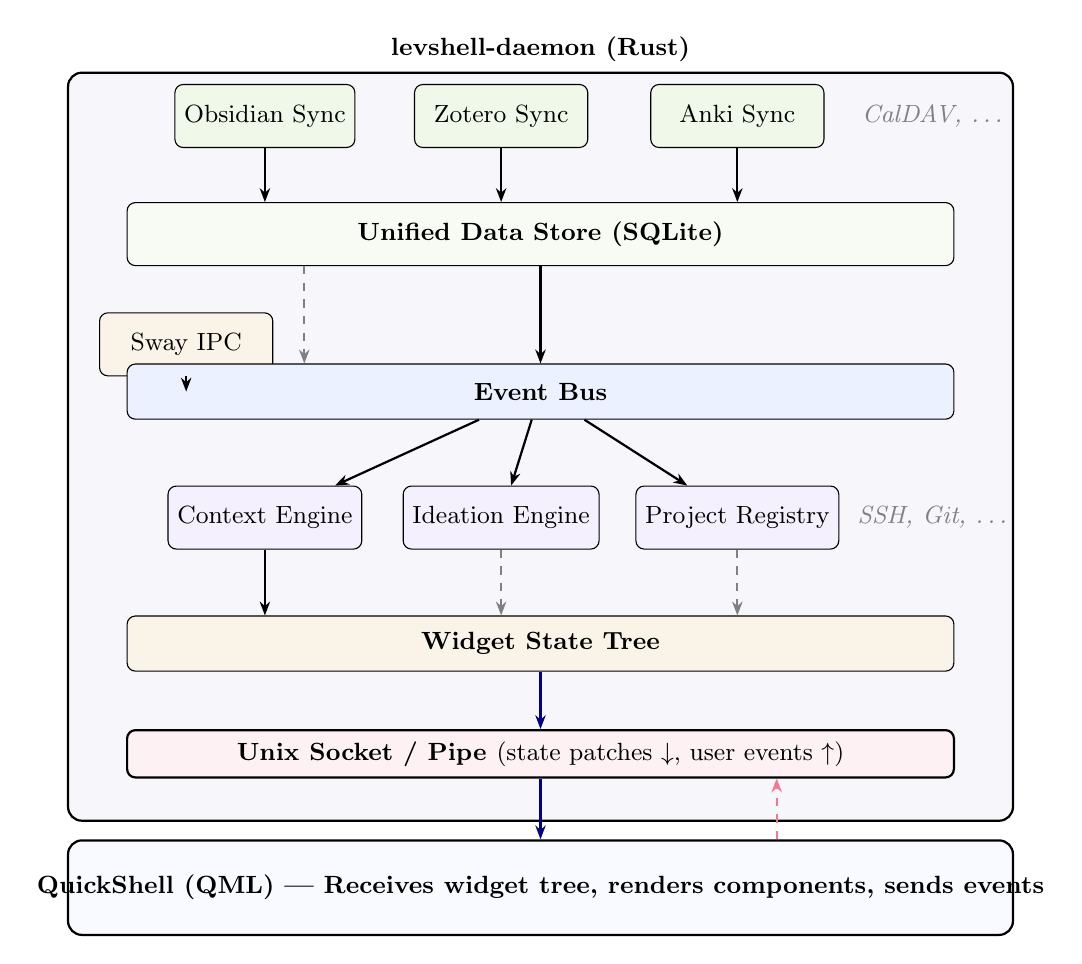
\begin{tikzpicture}[
  node distance=1.2cm and 1.5cm,
  box/.style={draw, rounded corners=3pt, minimum width=2.2cm, minimum height=0.8cm, font=\small},
  bigbox/.style={draw, rounded corners=5pt, thick, inner sep=10pt},
  arr/.style={-{Stealth[length=5pt]}, thick},
  bus/.style={draw, fill=levblue!15, rounded corners=3pt, minimum width=10.5cm, minimum height=0.7cm, font=\small\bfseries},
  >=Stealth
]

% Daemon boundary
\node[bigbox, minimum width=12cm, minimum height=9.5cm, fill=NavyBlue!3, label={[font=\bfseries\small]above:levshell-daemon (Rust)}] (daemon) at (0, -0.2) {};

% Sync adapters (top row) - external tools
\node[box, fill=levgreen!15] (obsidian) at (-3.5, 4) {Obsidian Sync};
\node[box, fill=levgreen!15] (zotero) at (-0.5, 4) {Zotero Sync};
\node[box, fill=levgreen!15] (anki) at (2.5, 4) {Anki Sync};
\node[font=\small\itshape\color{gray}] at (5, 4) {CalDAV, \ldots};

% Unified data store
\node[draw, fill=levgreen!8, rounded corners=3pt, minimum width=10.5cm, minimum height=0.8cm, font=\small\bfseries] (datastore) at (0, 2.5) {Unified Data Store (SQLite)};

% Sway IPC (separate from sync, direct to event bus)
\node[box, fill=levorange!15] (sway) at (-4.5, 1.1) {Sway IPC};

% Event bus
\node[bus] (eventbus) at (0, 0.5) {Event Bus};

% Processing modules (middle row)
\node[box, fill=levpurple!15] (context) at (-3.5, -1.1) {Context Engine};
\node[box, fill=levpurple!15] (ideation) at (-0.5, -1.1) {Ideation Engine};
\node[box, fill=levpurple!15] (projects) at (2.5, -1.1) {Project Registry};
\node[font=\small\itshape\color{gray}] at (5, -1.1) {SSH, Git, \ldots};

% Widget state tree
\node[bus, fill=levorange!15] (widgettree) at (0, -2.7) {Widget State Tree};

% Arrows from sync adapters to data store
\foreach \n in {obsidian, zotero, anki} {
  \draw[arr] (\n) -- (\n |- datastore.north);
}

% Arrows from data store to event bus (sync events)
\draw[arr] (datastore) -- (eventbus);

% Sway direct to event bus
\draw[arr] (sway) -- (sway |- eventbus.west);

% Arrows from bus to processors
\foreach \n in {context, ideation, projects} {
  \draw[arr] (eventbus) -- (\n);
}

% Processors also read from data store (dashed)
\draw[arr, dashed, gray] ([xshift=-3cm]datastore.south) -- ([xshift=-3cm]eventbus.north);

% Arrow from context to widget tree
\draw[arr] (context) -- (context |- widgettree.north);
\draw[arr, dashed, gray] (ideation) -- (ideation |- widgettree.north);
\draw[arr, dashed, gray] (projects) -- (projects |- widgettree.north);

% IPC channel
\node[draw, thick, fill=levred!10, rounded corners=3pt, minimum width=10.5cm, minimum height=0.6cm, font=\small\bfseries] (ipc) at (0, -4.1) {Unix Socket / Pipe \textnormal{(state patches $\downarrow$, user events $\uparrow$)}};

\draw[arr, thick, NavyBlue] (widgettree) -- (ipc);

% QuickShell
\node[bigbox, minimum width=12cm, minimum height=1.2cm, fill=levblue!5, label={[font=\bfseries\small]center:QuickShell (QML) --- Receives widget tree, renders components, sends events}] (qml) at (0, -5.8) {};

\draw[arr, thick, NavyBlue] (ipc) -- (qml);
\draw[arr, thick, levred, dashed] ([xshift=3cm]qml.north) -- ([xshift=3cm]ipc.south);

\end{tikzpicture}
\caption{High-level architecture of Levshell. Sync adapters populate the unified data store; modules operate on the data store via the event bus. The widget state tree drives the QML rendering layer over IPC.}
\label{fig:architecture}
\end{figure}


% ---------------------------------------------------------------------------
\subsection{IPC Protocol}
\label{sec:ipc}

The IPC channel between the daemon and QuickShell must satisfy four requirements: low latency (widget updates feel instant), structured messages (no string parsing), bidirectional communication (daemon pushes state; QML pushes user events), and incremental updates (patches, not full state retransmission).

\subsubsection{Transport}
A Unix domain socket carrying length-prefixed messages. The initial implementation uses JSON for the message format (QML/JavaScript parses JSON natively).

\subsubsection{Codec Abstraction and Serialization Strategy}

To allow migration to more efficient formats without protocol redesign, serialization is abstracted behind a codec interface:

\begin{lstlisting}[language={}]
trait Codec {
    fn encode(&self, msg: &Message) -> Result<Vec<u8>>;
    fn decode(&self, bytes: &[u8]) -> Result<Message>;
}
\end{lstlisting}

The v1 implementation uses \texttt{JsonCodec}. All message types are defined as Rust structs with \texttt{serde} derives, so switching to MessagePack is a single-line change (\texttt{serde\_json::to\_vec} $\to$ \texttt{rmp\_serde::to\_vec}). FlatBuffers requires schema files and a different access pattern but remains a viable future optimization.

\begin{notebox}[Payload Overhead Analysis]
In practice, most widget state changes are infrequent: workspace switches happen a few times per minute; SSH status updates every few seconds; Anki due counts change on review completion. High-frequency events (media progress, telemetry) produce at most 10--50 small messages per second. JSON parsing at this rate is microseconds of CPU work.

The dominant battery cost is \textbf{module polling overhead} (SSH latency checks, filesystem watchers, GPU monitoring), not IPC serialization. Accordingly, the daemon implements a global \textbf{power-aware mode}: when the system is on battery, all module poll intervals are automatically doubled (or set to a module-specific battery interval). This is configurable globally in \texttt{levshell.toml} and per-module in each module's configuration file.
\end{notebox}

\subsubsection{Daemon $\to$ QML: State Patches}
Each message is a targeted patch to the UI state. The daemon maintains a \textbf{widget state tree}---a tree of widget descriptors (type, properties, children, ordering, visibility). QML maintains a mirrored local state model and applies incoming patches reactively via QML property bindings. Example patch messages:

\begin{lstlisting}[language={}]
{ "op": "update", "path": "bar.left.ssh-dashboard",
  "state": { "connections": [...], "total_latency_ms": 42 } }

{ "op": "reorder", "path": "bar.left",
  "children": ["workspace-indicator", "ssh-dashboard", "git-status"] }

{ "op": "hide", "path": "bar.right.media-controls" }
\end{lstlisting}

\subsubsection{QML $\to$ Daemon: User Events}
Structured event messages sent when the user interacts with a widget:

\begin{lstlisting}[language={}]
{ "event": "widget_action", "widget": "ssh-dashboard",
  "action": "reconnect", "data": { "host": "gpu-cluster-3" } }

{ "event": "command_palette", "query": "zotero attention mechanisms" }

{ "event": "density_change", "mode": "compact" }
\end{lstlisting}

% ---------------------------------------------------------------------------
\subsection{Unified Data Model}
\label{sec:data-model}

The unified data model is the foundation of the hybrid architecture. It defines a shared schema for all research entities, independent of which external tool (if any) originally produced them. All shell logic---the context engine, ideation nudges, cross-tool queries, project tracking---operates exclusively on this model.

The data store is an embedded database within the daemon (SQLite for the initial implementation, chosen for its maturity, single-file simplicity, and excellent Rust support via \texttt{rusqlite}). The model is accessed by modules through a typed query API; modules never issue raw SQL.

\subsubsection{Core Entity Types}

\begin{lstlisting}[language={}]
Project {
    id: Uuid,
    name: String,
    status: Active | Simmering | Blocked | WritingUp | Complete,
    description: String,
    open_questions: Vec<OpenQuestion>,
    tags: Vec<String>,
    deadlines: Vec<Deadline>,
    collaborators: Vec<String>,
    accent_color: Option<String>,
    created_at: DateTime,
    updated_at: DateTime,
}

Note {
    id: Uuid,
    title: String,
    content: String,                  // Markdown
    tags: Vec<String>,
    links: Vec<Uuid>,                 // References to other Notes
    project_id: Option<Uuid>,
    source: SyncSource | Native,      // Provenance tracking
    created_at: DateTime,
    updated_at: DateTime,
}

Reference {
    id: Uuid,
    title: String,
    authors: Vec<String>,
    year: Option<u16>,
    venue: Option<String>,
    doi: Option<String>,
    citekey: String,
    abstract_text: Option<String>,
    tags: Vec<String>,
    collections: Vec<String>,
    pdf_path: Option<PathBuf>,
    reading_progress: Option<f32>,    // 0.0 to 1.0
    annotations: Vec<Annotation>,
    project_id: Option<Uuid>,
    source: SyncSource | Native,
    created_at: DateTime,
    updated_at: DateTime,
}

Flashcard {
    id: Uuid,
    front: String,
    back: String,
    tags: Vec<String>,
    linked_note: Option<Uuid>,
    linked_reference: Option<Uuid>,
    project_id: Option<Uuid>,
    // SRS scheduling state
    interval: Duration,
    ease_factor: f32,
    due_at: DateTime,
    review_count: u32,
    last_reviewed: Option<DateTime>,
    source: SyncSource | Native,
}

Event {
    id: Uuid,
    title: String,
    start: DateTime,
    end: DateTime,
    location: Option<String>,
    description: Option<String>,
    url: Option<String>,             // Video call link
    project_id: Option<Uuid>,
    recurrence: Option<RecurrenceRule>,
    reminders: Vec<ReminderOffset>,
    source: SyncSource | Native,
}

Task {
    id: Uuid,
    title: String,
    description: Option<String>,
    status: Pending | Active | Done | Cancelled,
    priority: Option<Priority>,
    due: Option<DateTime>,
    tags: Vec<String>,
    project_id: Option<Uuid>,
    source: SyncSource | Native,
}

Experiment {
    id: Uuid,
    name: String,
    project_id: Uuid,
    hypothesis: Option<String>,
    status: Queued | Running | Completed | Failed,
    host: Option<String>,            // SSH host where it ran
    git_hash: Option<String>,
    config: Option<serde_json::Value>,
    metrics: HashMap<String, f64>,
    started_at: Option<DateTime>,
    completed_at: Option<DateTime>,
    notes: Option<String>,
    source: SyncSource | Native,
}
\end{lstlisting}

\subsubsection{Provenance Tracking}

Every entity carries a \texttt{source} field that records its origin:

\begin{lstlisting}[language={}]
enum DataSource {
    Native,                          // Created within Levshell
    SyncSource {
        provider: String,            // "zotero", "obsidian", "anki", ...
        external_id: String,         // ID in the source system
        last_synced: DateTime,
        sync_direction: Bidirectional | ImportOnly | ExportOnly,
    },
}
\end{lstlisting}

This enables several critical behaviors: the sync engine knows which entities to push back to external tools (for bidirectional sync), the system can detect and resolve conflicts when both sides have been modified, and when a native component replaces a sync adapter, all existing entities remain valid---only their \texttt{source} field changes from \texttt{SyncSource} to \texttt{Native} once the external tool is no longer the authority.

\subsubsection{Cross-Entity Relations}

The data model supports typed links between entities:

\begin{itemize}[leftmargin=1.5em, itemsep=2pt]
  \item A \texttt{Note} can link to other \texttt{Note}s (knowledge graph), to \texttt{Reference}s (literature notes), and to a \texttt{Project}.
  \item A \texttt{Flashcard} can link to the \texttt{Note} or \texttt{Reference} it was derived from.
  \item An \texttt{Experiment} links to its \texttt{Project} and optionally to \texttt{Note}s and \texttt{Reference}s.
  \item A \texttt{Reference}'s annotations can be automatically scaffolded into \texttt{Note}s.
  \item A \texttt{Flashcard}'s review performance can be surfaced on its linked \texttt{Note} as a confidence signal.
\end{itemize}

These cross-entity relations are what make the unified model fundamentally more powerful than a collection of isolated tools. The query ``show me everything related to project X'' is a single indexed database query, not a multi-source aggregation job.

\subsubsection{Sync Engine}

The sync engine is a daemon subsystem that runs sync adapters on configurable intervals. Each adapter implements a common sync trait:

\begin{lstlisting}[language={}]
trait SyncAdapter {
    fn name(&self) -> &str;
    fn entity_types(&self) -> Vec<EntityType>;  // What it syncs
    fn pull(&self, since: DateTime) -> Result<Vec<SyncDelta>>;
    fn push(&self, deltas: Vec<SyncDelta>) -> Result<()>;
    fn full_import(&self) -> Result<Vec<Entity>>;
    fn status(&self) -> SyncStatus;  // Healthy, Stale, Error
}
\end{lstlisting}

Sync operates on deltas: on each pull, the adapter fetches entities modified since the last sync timestamp and upserts them into the unified store. Conflict resolution follows a last-write-wins strategy with optional manual resolution for detected conflicts. The sync engine emits events on the event bus (\texttt{SyncCompleted}, \texttt{SyncConflict}, \texttt{SyncError}) so modules can react.

\begin{notebox}[Initial Sync Adapters]
The v1 implementation targets sync adapters for: Zotero (SQLite database read + optional Zotero API for remote libraries), Obsidian (filesystem watcher on vault directory), AnkiConnect (HTTP JSON-RPC), and CalDAV (for calendar sync with Google Calendar, Nextcloud, etc.). Additional adapters for Taskwarrior, W\&B, and SLURM are planned as subsequent additions.
\end{notebox}

\subsubsection{Migration Path: Sync Adapter to Native Component}

When a native component is ready to replace a sync adapter, the migration follows a defined sequence:

\begin{enumerate}[leftmargin=1.5em, itemsep=2pt]
  \item The native component is activated alongside the sync adapter in a read-only overlap period. Both populate the unified model; the native component is used for display and interaction, while the sync adapter continues to pull updates from the external tool.
  \item The user migrates their workflow to the native component (e.g., creates new notes in Levshell's knowledge base instead of Obsidian).
  \item Once the user is satisfied, the sync adapter is deactivated. Existing entities in the unified model remain unchanged---they simply stop receiving updates from the external tool. The \texttt{source} field is optionally migrated from \texttt{SyncSource} to \texttt{Native}.
  \item An export function remains available so data can be pushed back to the external tool's format at any time (e.g., export the knowledge base as an Obsidian-compatible vault of Markdown files).
\end{enumerate}

At every stage, the system is fully functional. No step requires downtime or data loss.


% ---------------------------------------------------------------------------
\subsection{Module System}
\label{sec:modules}

Every feature is implemented as a \textbf{module} within the daemon. A module is defined by a Rust trait (with a future path to out-of-process modules over IPC for extensibility in other languages).

\subsubsection{Module Trait}

A module provides the following interface:

\begin{lstlisting}[language={}]
Module {
    name()        -> &str              // Identity
    widgets()     -> Vec<WidgetDescriptor>  // What it can render
    relevance()   -> Vec<RelevanceRule>     // When to show/hide
    config_schema() -> ConfigSchema         // Configurable parameters
    on_event(Event)                         // React to bus events
    tick()                                  // Periodic poll (optional)
    start() / stop()                        // Lifecycle
}
\end{lstlisting}

\subsubsection{Module Isolation}
Modules do not reference each other directly. All inter-module communication flows through the \textbf{event bus}---a typed publish/subscribe system internal to the daemon.

\subsubsection{Out-of-Process Modules}
An external binary speaking the module protocol over a Unix socket or stdio. The daemon treats it identically to an in-process module from a protocol perspective. This enables modules written in Python, Go, or any language.

\paragraph{Security and Permission Model.}
Out-of-process modules running as native binaries on the user's system have the same OS-level privileges as the user. This is consistent with every existing Linux desktop extension system (Polybar modules, GNOME Shell extensions, etc.) but must be mitigated through layered defenses:

\begin{enumerate}[leftmargin=1.5em, itemsep=4pt]
  \item \textbf{Tier 1 --- Capability manifests.} Every out-of-process module ships a manifest declaring what it needs: filesystem paths, network access, specific IPC buses, environment variables. The daemon presents this manifest to the user at install time (analogous to mobile app permissions). This does not enforce restrictions at the OS level but creates a social contract and makes malicious intent visible through review.

  \item \textbf{Tier 2 --- Protocol-level restriction.} The module IPC protocol limits what a module can \emph{ask the daemon to do}. A module can push widget state updates and subscribe to events---it cannot, through the protocol, read arbitrary files, access other modules' internal state, or invoke arbitrary daemon functions. A compromised module can display misleading widgets and receive its subscribed events, but cannot exfiltrate data \emph{through the daemon}.

  \item \textbf{Tier 3 --- WebAssembly sandboxing (recommended for community extensions).} For extensions from untrusted authors, the daemon offers a Wasm runtime (Wasmtime or Wasmer) as an alternative execution environment. Wasm modules run with \emph{only} the capabilities the daemon explicitly grants via WASI---specific filesystem paths, specific network endpoints, nothing else. The tradeoff is reduced capability (no arbitrary system calls, no process spawning), but this is genuine sandboxing and is sufficient for most widget types.

  \item \textbf{Tier 4 --- OS-level confinement (optional hardening).} For native out-of-process modules, the daemon can optionally launch them under a restrictive AppArmor or Landlock profile that limits filesystem access, network access, and Linux capability usage. This requires system-level configuration but provides defense-in-depth for security-conscious users.
\end{enumerate}

\begin{notebox}[v1 Recommendation]
Ship with Tier~1 (manifests) and Tier~2 (protocol restriction). Implement Tier~3 (Wasm) as the recommended and documented path for community extensions. Tier~4 (AppArmor/Landlock) is a hardening option for future releases. The threat model should be documented honestly: native out-of-process modules are trusted code.
\end{notebox}

\subsubsection{QML Widget Skins}
The daemon specifies widget type and state; the QML side has a component file for each widget type. Users can override QML components to customize appearance without modifying the daemon.


% ---------------------------------------------------------------------------
\subsection{Context Engine}
\label{sec:context-engine}

The context engine is the subsystem that makes Levshell adaptive. It runs inside the daemon and is responsible for deciding which widgets are visible, where, and at what prominence level.

\subsubsection{Input Signals}

\begin{longtable}{p{4.5cm} p{9cm}}
\toprule
\textbf{Signal} & \textbf{Source} \\
\midrule
Active workspace & Sway IPC subscription \\
Focused window (app\_id, class, title) & Sway IPC subscription \\
Open windows per workspace & Sway IPC subscription \\
Time of day, day of week & System clock \\
Focus session state & Pomodoro / session timer module \\
Active context profile & Manual selection or auto-trigger rules \\
Associated project & Workspace configuration or inference \\
Module-specific conditions & Each module's internal state (e.g., ``active SSH connections $> 0$'') \\
\bottomrule
\end{longtable}

\subsubsection{Resolution Layers}

The context engine resolves widget layout through four layers, applied in order:

\begin{enumerate}[leftmargin=1.5em, itemsep=4pt]
  \item \textbf{Base layer.} A default widget layout that always applies: clock, workspace indicator, system tray, notification icon. This is the fallback when no context-specific rules match.

  \item \textbf{Module relevance scores.} Each module declares relevance rules as predicates. Rules specify conditions under which a widget should be visible, compact, expanded, or hidden. Conditions reference input signals and module-internal state.

  \item \textbf{Context profiles.} Named bundles of relevance overrides. A ``writing'' profile might expand citation search, show word count, hide media controls, and suppress notifications. Profiles are activated manually, by keybind, or by auto-trigger rules.

  \item \textbf{User override.} A keybind always toggles to the base layer or a ``show everything'' mode, guaranteeing that context-aware hiding never locks the user out of any widget.
\end{enumerate}

\subsubsection{Relevance Rule Format}

Relevance rules are declared in module configuration files using a predicate DSL:

\begin{lstlisting}[language={}]
# Example: ssh-monitor module relevance
[relevance.ssh-dashboard]
default = "hidden"

[[relevance.ssh-dashboard.when]]
condition = "self.active_connections > 0"
prominence = "visible:compact"

[[relevance.ssh-dashboard.when]]
workspace_tag = "remote"
prominence = "expanded"
\end{lstlisting}

\subsubsection{Conflict Resolution Algorithm}

Widget prominence is resolved by a strict, deterministic cascade. Given the same input signals, the algorithm always produces the same output. The prominence levels form a total order: \texttt{hidden} $<$ \texttt{icon-only} $<$ \texttt{compact} $<$ \texttt{visible} $<$ \texttt{expanded}.

\begin{enumerate}[leftmargin=1.5em, itemsep=4pt]
  \item \textbf{Step 1 --- Base layout.} Every widget slot is assigned its default prominence from the base layer configuration. This produces a complete, valid layout with no gaps or conflicts.

  \item \textbf{Step 2 --- Module relevance rules.} For each widget, evaluate its owning module's relevance predicates against the current context signals. If any predicate matches, its specified prominence \emph{replaces} the base layer value. If multiple predicates within the same module match (e.g., both ``active SSH connections $> 0$'' and ``workspace tagged remote''), the \emph{most prominent} matching value wins. This is well-defined because prominence is a total order.

  \item \textbf{Step 3 --- Active context profile.} If a context profile is active (e.g., ``writing mode''), its explicit overrides replace all previous values for the widgets it mentions. Profiles are user-authored and always take precedence over module self-assessment. Widgets not mentioned in the active profile retain their Step~2 values.

  \item \textbf{Step 4 --- Spatial constraint enforcement.} The bar has a finite pixel budget. Walk the widget list in \emph{global priority order} (a user-configurable ordered list that ships with sensible defaults). Place each widget at its resolved prominence. If placing a widget at its current prominence would overflow the available space, demote it one level (e.g., \texttt{expanded} $\to$ \texttt{compact} $\to$ \texttt{icon-only} $\to$ \texttt{hidden}). Highest-priority widgets receive first claim on bar real estate. This is a greedy $O(n)$ algorithm.

  \item \textbf{Step 5 --- User override.} If the user has explicitly pinned or hidden a widget via keybind or manual toggle, that decision is absolute and overrides all previous steps. A global ``show everything'' keybind sets all widgets to \texttt{visible}, bypassing the entire cascade.
\end{enumerate}

\subsubsection{Hysteresis and Flicker Prevention}

To prevent visual instability when a condition oscillates around a threshold (e.g., CPU hovering at 59--61\% around a 60\% trigger), the context engine applies \textbf{hysteresis} to all condition-driven visibility changes:

\begin{itemize}[leftmargin=1.5em, itemsep=2pt]
  \item A condition must be continuously true for a minimum \textbf{activation delay} (default: 2 seconds) before it triggers a visibility change.
  \item Once activated, a condition must be continuously false for a longer \textbf{deactivation delay} (default: 10 seconds) before the change reverts.
  \item Both delays are configurable per-rule.
\end{itemize}

This ensures the bar layout is stable even when underlying signals are noisy. The computational cost is negligible: one timestamp comparison per active rule per evaluation cycle.


% ---------------------------------------------------------------------------
\subsection{Event Bus}
\label{sec:event-bus}

The event bus is the internal communication backbone of the daemon. Modules publish typed events and subscribe to events from other modules or from core subsystems.

\subsubsection{Example Event Types}

\begin{lstlisting}[language={}]
WorkspaceChanged     { name, focused_window }
SSHConnectionEstablished  { host, pid, workspace }
SSHConnectionDropped { host, reason }
AnkiDueCountChanged  { total, by_tag: HashMap }
FocusSessionStarted  { project, duration }
FocusSessionEnded    { project, actual_duration }
IdleDetected         { duration }
FileModified         { path }
GitCommitPushed      { repo, branch, hash }
ExperimentStatusUpdate  { id, host, metrics }
ZoteroItemAdded      { key, title, authors, tags }
ObsidianNoteModified { path, title, tags, links }
NudgeDelivered       { project, question }
ProfileActivated     { name }
\end{lstlisting}

Any module can subscribe to any event type. The ideation engine subscribes broadly to maintain situational awareness. The context engine subscribes to events that affect widget layout. New modules subscribe only to the events they need, and publishing a new event type never requires changes to existing modules.

% ---------------------------------------------------------------------------
\subsection{Project Registry}
\label{sec:project-registry}

The project registry is a core daemon service that provides indexed access to \texttt{Project} entities in the unified data model (Section~\ref{sec:data-model}). It is not a module itself but a shared service that modules query. Projects are the fundamental unit of research context: they link notes, references, flashcards, experiments, tasks, and events into coherent research threads.

Projects can be created natively within Levshell or seeded from TOML configuration files under \texttt{\textasciitilde/.config/levshell/projects/}. Configuration-defined projects are loaded into the unified data store on startup and are hot-reloadable via \texttt{inotify}. The project registry also maintains runtime metadata not persisted in the data store: which workspaces are currently associated with each project, accumulated focus time for the current session, and the last-active timestamp.

In addition to the project entity fields defined in the unified data model, the registry tracks external system associations that are relevant to context inference but not part of the core data model:

\begin{lstlisting}[language={}]
ProjectConfig {              // From TOML, merged with DB entity
    git_repos: Vec<PathBuf>,
    ssh_hosts: Vec<String>,
    workspace_names: Vec<String>,
    accent_color: Option<String>,
}
\end{lstlisting}

% ---------------------------------------------------------------------------
\subsection{App-to-Context Mapping}
\label{sec:app-context}

The system maps running applications to contextual tags at three levels of user effort:

\begin{enumerate}[leftmargin=1.5em, itemsep=4pt]
  \item \textbf{Zero-effort defaults.} Levshell ships with a built-in mapping of common Wayland \texttt{app\_id} values to context tags. For example: \texttt{org.pwmt.zathura} $\to$ \texttt{pdf-reader}; \texttt{com.obsidian} $\to$ \texttt{knowledge-base}; \texttt{Alacritty} $\to$ \texttt{terminal}.

  \item \textbf{One-line configuration.} Users add custom mappings in a configuration file:
  \begin{lstlisting}[language={}]
[apps.window-rules]
"org.texstudio" = { tags = ["latex", "writing"] }
"firefox" = { tags = ["browser"], context = "neutral" }
"slack" = { tags = ["communication"] }
  \end{lstlisting}

  \item \textbf{Workspace declarations.} Workspaces can be pre-declared with intent, so context is known before any window is inspected:
  \begin{lstlisting}[language={}]
[workspaces.research-llm]
tags = ["research", "coding", "remote"]
project = "llm-alignment"
accent-color = "#7aa2f7"
  \end{lstlisting}
\end{enumerate}


% ---------------------------------------------------------------------------
\subsection{Configuration Architecture}
\label{sec:config}

All configuration lives under \texttt{\textasciitilde/.config/levshell/} and is hot-reloadable via \texttt{inotify}. No daemon restart is required for configuration changes.

\subsubsection{Directory Structure}

\begin{lstlisting}[language={}]
~/.config/levshell/
  levshell.toml            # Global: theme, bar density, keybinds
  modules/
    ssh-monitor.toml       # SSH module config
    ideation.toml          # Nudge intervals, settings
    ...
  sync/
    zotero.toml            # Zotero sync adapter config
    obsidian.toml          # Obsidian sync adapter config
    anki.toml              # AnkiConnect sync adapter config
    caldav.toml            # CalDAV sync adapter config
    ...
  projects/
    llm-alignment.toml
    distributed-consensus.toml
    ...
  profiles/
    writing.toml           # Context profile overrides
    debugging.toml
    reading.toml
    ...
  rules/
    app-tags.toml          # Window class -> tag mappings
    auto-profiles.toml     # Condition -> profile triggers
  themes/
    catppuccin-mocha.toml
    ...

~/.local/share/levshell/
  levshell.db              # Unified data store (SQLite)
  levshell.db-wal          # Write-ahead log
  assets/                  # Attached images, PDFs, etc.
\end{lstlisting}

\subsubsection{Configuration Precedence}
Module defaults $<$ module config file $<$ context profile overrides $<$ user keybind override. Each layer can only narrow or override; it cannot disable the user's ability to manually override.


% ---------------------------------------------------------------------------
\subsection{Extension Points}
\label{sec:extensions}

\begin{longtable}{p{4cm} p{9.5cm}}
\toprule
\textbf{Extension Point} & \textbf{Description} \\
\midrule
Out-of-process modules & External binaries speaking the module protocol over Unix socket or stdio. Enables modules in any language. \\
QML widget skins & User-overridable QML component files for each widget type. Separates logic from presentation. \\
Scripting layer & Lua (via \texttt{mlua}) or Wasm for complex relevance rules and custom logic beyond static configuration. \\
Command palette providers & Any module or external script can register itself as a search provider in the command palette. \\
Trigger system actions & User-defined event $\to$ action rules, extensible with custom event types from out-of-process modules. \\
Theme packages & Distributable theme bundles containing color definitions, font specifications, and optional QML overrides. \\
\bottomrule
\end{longtable}


% ===========================================================================
\section{Implementation Decisions}
\label{sec:impl-decisions}

This section records the concrete technology choices and design decisions that govern the implementation. These are locked down prior to coding and should not be revisited without strong justification.

% ---------------------------------------------------------------------------
\subsection{Rust Workspace Layout}
\label{sec:workspace-layout}

The daemon is a Cargo workspace using a \textbf{layered crate split}. Crates are organized by architectural layer, not by feature. The dependency graph flows strictly downward---no cycles are permitted.

\begin{lstlisting}[language={}]
levshell/
  Cargo.toml                  # Workspace root
  crates/
    levshell-core/            # Event bus, module trait, module runner,
                              # health state management
    levshell-data/            # Unified data model, SQLite schema,
                              # query API, migrations, FTS5
    levshell-ipc/             # Codec trait, message types,
                              # Unix socket server/client
    levshell-context/         # Context engine, relevance rules,
                              # profiles, hysteresis
    levshell-sync/            # SyncAdapter trait, sync engine,
                              # individual adapters (Zotero, Obsidian, ...)
    levshell-config/          # Layered config loading, file watching,
                              # config struct definitions
    levshell-modules/         # All built-in shell modules
    levshell-daemon/          # Binary crate: main(), wires everything,
                              # lifecycle management
  shell/                      # QuickShell QML
    main.qml
    components/               # Shared QML components (degraded-state
                              # wrapper, animations, theme bindings)
    widgets/                  # Per-widget-type QML components
  config/                     # Default and example configuration files
  spec/                       # This specification document
\end{lstlisting}

\subsubsection{Crate Dependency Graph}

\begin{figure}[h]
\centering
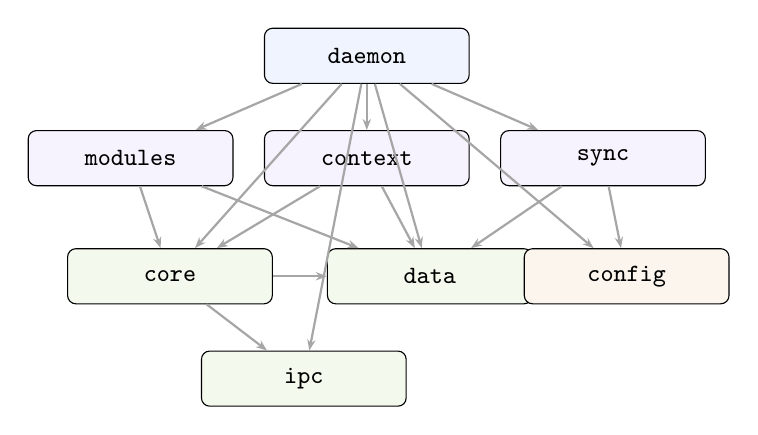
\begin{tikzpicture}[
  node distance=1.0cm and 1.8cm,
  box/.style={draw, rounded corners=3pt, minimum width=2.6cm, minimum height=0.7cm, font=\small\ttfamily, fill=#1},
  arr/.style={-{Stealth[length=4pt]}, thick, gray!70},
  >=Stealth
]

\node[box=levblue!12] (daemon) at (0, 0) {daemon};
\node[box=levpurple!12] (modules) at (-3, -1.3) {modules};
\node[box=levpurple!12] (context) at (0, -1.3) {context};
\node[box=levpurple!12] (sync) at (3, -1.3) {sync};
\node[box=levgreen!12] (core) at (-2.5, -2.8) {core};
\node[box=levgreen!12] (data) at (0.8, -2.8) {data};
\node[box=levgreen!12] (ipc) at (-0.8, -4.1) {ipc};
\node[box=levorange!12] (config) at (3.3, -2.8) {config};

\draw[arr] (daemon) -- (modules);
\draw[arr] (daemon) -- (context);
\draw[arr] (daemon) -- (sync);
\draw[arr] (daemon) -- (core);
\draw[arr] (daemon) -- (data);
\draw[arr] (daemon) -- (ipc);
\draw[arr] (daemon) -- (config);
\draw[arr] (modules) -- (core);
\draw[arr] (modules) -- (data);
\draw[arr] (context) -- (core);
\draw[arr] (context) -- (data);
\draw[arr] (sync) -- (data);
\draw[arr] (sync) -- (config);
\draw[arr] (core) -- (ipc);
\draw[arr] (core) -- (data);

\end{tikzpicture}
\caption{Crate dependency graph. All arrows point from dependent to dependency. The \texttt{daemon} crate (binary) depends on everything; leaf crates (\texttt{ipc}, \texttt{data}, \texttt{config}) have no internal dependencies.}
\label{fig:crate-deps}
\end{figure}

\subsubsection{Rationale}
This split provides compile parallelism where it matters most: \texttt{levshell-data} and \texttt{levshell-ipc} change rarely once stable, so downstream crates avoid unnecessary recompilation during module iteration. The layered boundaries enforce the architectural invariant that modules cannot import sync adapter internals and the context engine cannot reach into module state. If \texttt{levshell-modules} grows too large, individual modules can be extracted into their own crates without affecting other layers.

Sync adapters live as Rust modules within \texttt{levshell-sync}. The \texttt{SyncAdapter} trait is defined in \texttt{levshell-data} so that native components (in \texttt{levshell-modules}) can write to the data store without depending on \texttt{levshell-sync}.


% ---------------------------------------------------------------------------
\subsection{Database and Schema Decisions}
\label{sec:db-decisions}

\begin{longtable}{p{4.5cm} p{9cm}}
\toprule
\textbf{Decision} & \textbf{Choice and Rationale} \\
\midrule
Schema approach & \textbf{Hybrid relational + JSON.} Core queryable fields (title, status, project\_id, citekey, due\_at) are proper columns with indexes. Variable-shape data (annotations, experiment metrics, custom metadata) is stored as JSON in \texttt{TEXT} columns. This gives fast indexed queries on the hot paths while accommodating evolving data shapes without constant migrations. \\
\addlinespace
Tags & \textbf{Polymorphic join table.} A single \texttt{entity\_tags(entity\_id BLOB, entity\_type TEXT, tag TEXT)} table with indexes on \texttt{(tag)} and \texttt{(entity\_id, entity\_type)}. Tag-based queries (``all entities tagged X,'' tag overlap between projects) are fundamental to the ideation engine and context engine; the query penalty of JSON arrays is unacceptable. \\
\addlinespace
Entity IDs & \textbf{UUID v7, stored as BLOB(16).} Globally unique (essential for sync adapters generating IDs before insertion), time-ordered (B-tree indexes maintain temporal locality for recent-data queries), and compact (16 bytes vs.\ 36 for TEXT representation). Generated via the Rust \texttt{uuid} crate with v7 support. \\
\addlinespace
Relations & \textbf{Explicit FKs + generic relation table.} Primary, well-known relations (flashcard $\to$ note, experiment $\to$ project, note/reference/task/event $\to$ project) use nullable foreign key columns with indexes. The knowledge graph (note $\to$ note backlinks) and citation graph (reference $\to$ reference) use a generic \texttt{entity\_relations(source\_id, source\_type, target\_id, target\_type, relation\_kind)} table. \\
\addlinespace
Provenance & \textbf{Separate \texttt{sync\_metadata} table.} Entity tables carry only domain data. Sync provenance (provider name, external ID, last synced timestamp, sync direction, sync hash) lives in \texttt{sync\_metadata(entity\_id, entity\_type, ...)}. Keeps entity tables clean; enables efficient sync-engine-wide queries. \\
\addlinespace
Full-text search & \textbf{FTS5 initially.} FTS5 virtual tables shadow the \texttt{notes} and \texttt{references} tables, maintained via triggers. The query API abstracts over the search backend so Tantivy can be substituted later if needed. \\
\addlinespace
Migrations & \textbf{\texttt{rusqlite\_migration}.} Migrations are embedded as SQL string constants in the \texttt{levshell-data} crate, applied transactionally on daemon startup. \\
\addlinespace
WAL mode & \textbf{Enabled.} \texttt{PRAGMA journal\_mode=WAL} is set on database open for concurrent read/write performance. \\
\bottomrule
\end{longtable}


% ---------------------------------------------------------------------------
\subsection{Runtime and Library Decisions}
\label{sec:runtime-decisions}

\begin{longtable}{p{4.5cm} p{9cm}}
\toprule
\textbf{Decision} & \textbf{Choice and Rationale} \\
\midrule
Async runtime & \textbf{Tokio} (multi-threaded, small thread pool of 2--4). Required by key dependencies: \texttt{swayipc} (Sway IPC), \texttt{reqwest} (HTTP for AnkiConnect, W\&B, arXiv), \texttt{tokio-tungstenite} (WebSocket, if needed). Fighting the ecosystem for an alternative runtime is not justified. \\
\addlinespace
SQLite binding & \textbf{\texttt{rusqlite} + \texttt{tokio::task::spawn\_blocking}.} \texttt{rusqlite} is the most mature Rust SQLite binding. SQLite is inherently synchronous; any ``async'' wrapper does the same \texttt{spawn\_blocking} under the hood. The \texttt{levshell-data} crate exposes an async API externally while using synchronous \texttt{rusqlite} internally. \\
\addlinespace
Event bus & \textbf{Custom fan-out over \texttt{tokio::sync::mpsc}.} Each subscriber gets its own bounded \texttt{mpsc} channel. The bus receives events and fans them out to subscriber channels, with per-subscriber filtering (modules only receive events they subscribed to). Slow consumers receive a log warning and dropped events rather than blocking the publisher. Events use a typed Rust enum (all types known at compile time for in-process modules). 50--100 lines of code atop \texttt{tokio::sync::mpsc}. \\
\addlinespace
Configuration & \textbf{Dedicated \texttt{levshell-config} crate} using the \texttt{config} crate for layered configuration (files, environment variables, defaults) with \texttt{serde} deserialization. File watching via the \texttt{notify} crate for hot-reload. Config structs derive \texttt{serde::Deserialize} and are loaded from TOML files. \\
\addlinespace
Error handling & \textbf{\texttt{thiserror} in library crates, \texttt{anyhow} in the binary.} Library crates define typed error enums (\texttt{DataError}, \texttt{SyncError}, \texttt{IpcError}, \texttt{ContextError}) enabling programmatic error matching. The \texttt{levshell-daemon} binary uses \texttt{anyhow} for top-level error propagation. \\
\addlinespace
Serialization & \textbf{\texttt{serde} + \texttt{serde\_json}} for IPC messages and JSON columns. The codec abstraction trait (Section~\ref{sec:ipc}) enables future migration to MessagePack (\texttt{rmp-serde}) without protocol changes. \\
\addlinespace
UUID generation & \textbf{\texttt{uuid} crate} with v7 feature flag. \\
\bottomrule
\end{longtable}


% ---------------------------------------------------------------------------
\subsection{IPC Message Types (Phase 0)}
\label{sec:ipc-messages}

The initial IPC protocol defines the minimum set of messages required for the first end-to-end module.

\subsubsection{Daemon $\to$ QML}

\begin{lstlisting}[language={}]
WidgetUpdate {
    widget_id: String,
    widget_type: String,
    state: serde_json::Value,     // Widget-specific, opaque to IPC
    status: WidgetStatus,         // Normal | Stale | Error | Unavailable
}

WidgetVisibility {
    widget_id: String,
    visible: bool,
    prominence: Prominence,       // Hidden | IconOnly | Compact | Visible
                                  //   | Expanded
}

BarLayout {
    left: Vec<String>,            // Ordered widget IDs
    center: Vec<String>,
    right: Vec<String>,
}
\end{lstlisting}

\subsubsection{QML $\to$ Daemon}

\begin{lstlisting}[language={}]
WidgetAction {
    widget_id: String,
    action: String,
    data: serde_json::Value,      // Action-specific payload
}

CommandPaletteQuery {
    query: String,
}

CommandPaletteSelect {
    provider: String,
    item_id: String,
}

DensityChange {
    mode: BarDensity,             // Full | Compact | Hidden
}
\end{lstlisting}

Using \texttt{serde\_json::Value} for state and action payloads is deliberate: it keeps the IPC crate agnostic to specific widget state shapes. Each widget type defines its own state struct in the modules crate, serializes it for IPC, and the QML side parses it according to the widget type.


% ===========================================================================
\section{Architectural Constraints \& Failure Modes}
\label{sec:constraints}

This section addresses known architectural risks and defines the strategies for mitigating them. These constraints are as fundamental to the design as the feature set itself.

% ---------------------------------------------------------------------------
\subsection{Integration Brittleness and Sync Adapter Isolation}
\label{sec:provider-layer}

During the hybrid phase, Levshell relies on sync adapters to import data from third-party tools (Obsidian, Zotero, AnkiConnect, Taskwarrior, etc.) into the unified data model. Each of these tools may change its database schema, API surface, or file format between versions. Sync adapters are therefore the most maintenance-intensive and fragile layer of the system.

\subsubsection{Design Constraint: Modules Never Touch External Tools}

All shell modules operate exclusively on the unified data model (Section~\ref{sec:data-model}). No module ever queries Zotero's SQLite database, parses Obsidian's Markdown, or calls AnkiConnect's HTTP API. Tool-specific code is confined entirely to sync adapter implementations, which are isolated, independently testable, and replaceable.

This means that when a sync adapter breaks due to an upstream change, the impact is contained: the affected entity types stop receiving updates (the sync engine emits \texttt{SyncError} events and the corresponding widgets transition to \texttt{Stale}), but all existing data in the unified model remains valid, all other modules and adapters continue operating normally, and the user can continue working with the last-known-good state while the adapter is repaired.

\subsubsection{Sync Adapter Inventory}

\begin{longtable}{p{3.8cm} p{3.5cm} p{3.5cm} p{2.7cm}}
\toprule
\textbf{Entity Type} & \textbf{Initial Adapter} & \textbf{Alt.\ Adapters} & \textbf{Native Target} \\
\midrule
References & Zotero (SQLite + API) & BibTeX file & Levshell Refs \\
Notes & Obsidian (filesystem) & Logseq, plain MD & Levshell KB \\
Flashcards & AnkiConnect (HTTP) & Mochi & Levshell SRS \\
Events & CalDAV & Google API & Levshell Cal \\
Tasks & Taskwarrior (CLI) & Todoist API & Levshell Tasks \\
Experiments & W\&B (API) & MLflow & Levshell Lab \\
Jobs & SLURM (CLI) & PBS/Torque & --- \\
\bottomrule
\end{longtable}

The ``Native Target'' column indicates the planned native component that will eventually replace each sync adapter. Components marked ``---'' are expected to remain as sync adapters indefinitely, as they interface with external infrastructure (e.g., HPC clusters) rather than personal data stores.

\subsubsection{Version Probing}

On startup, each sync adapter performs a \textbf{version probe}: it checks the tool's database schema version, API version, or binary version and logs a warning if the detected version is unrecognized. This provides early detection of incompatible upstream changes rather than silent data corruption or cryptic runtime errors.

\subsubsection{Long-Term Brittleness Reduction}

The hybrid architecture provides a natural path to reducing integration brittleness over time. As each native component matures and replaces its corresponding sync adapter, the number of external tool dependencies decreases. The end state---a fully native suite---has \emph{zero} sync adapter brittleness. The migration sequence should prioritize replacing the adapters with the highest maintenance burden and most frequent upstream breakage first.


% ---------------------------------------------------------------------------
\subsection{Widget Degraded State and Error Handling UI}
\label{sec:degraded-state}

When an external integration fails---a network request times out, a database query returns an error, a CLI tool is not installed---the user must never be left wondering whether the shell is frozen or working. Every widget supports four visual states, managed uniformly by the daemon's module runner.

\subsubsection{Widget Health States}

\begin{longtable}{p{2.5cm} p{3.5cm} p{7.5cm}}
\toprule
\textbf{State} & \textbf{Visual Treatment} & \textbf{Semantics} \\
\midrule
\texttt{Normal} & Default appearance & Data is fresh; the backing integration is healthy. \\
\texttt{Stale} & Data slightly dimmed; small clock icon & The last successful fetch was longer ago than expected. The widget displays last-known-good data but signals that it may be outdated. \\
\texttt{Error} & Compact warning icon; tooltip with message & The module encountered an identifiable failure. Tooltip shows the error (``SLURM query timed out,'' ``AnkiConnect not running''). Click offers retry or settings link. \\
\texttt{Unavailable} & Widget hidden entirely & The module's backing service is not configured or not installed. No visual noise for unconfigured features. \\
\bottomrule
\end{longtable}

\subsubsection{Automatic State Transitions}

The daemon's module runner wraps every module's external calls with a timeout and a staleness tracker. State transitions are managed by the runner, not by individual modules:

\begin{itemize}[leftmargin=1.5em, itemsep=2pt]
  \item If a module's \texttt{tick()} or provider call has not successfully updated a widget's state within $2\times$ the expected poll interval, the widget transitions to \texttt{Stale} automatically.
  \item If a call returns an explicit error, the widget transitions to \texttt{Error} with the error message attached.
  \item If the configured provider is absent or returns a ``not installed'' probe result, the widget is set to \texttt{Unavailable} at startup and excluded from layout calculations.
  \item A successful update always resets the state to \texttt{Normal}.
\end{itemize}

\subsubsection{QML-Side Consistency}

On the rendering side, every widget component receives a \texttt{status} field alongside its data payload: \texttt{"normal"}, \texttt{"stale"}, \texttt{"error"}, or \texttt{"unavailable"}. A shared QML wrapper component implements the standard visual treatment for non-normal states, ensuring consistent degraded-state language across the entire bar. Individual widget components do not need to implement error handling themselves.


% ---------------------------------------------------------------------------
\subsection{Power Awareness}
\label{sec:power-awareness}

The daemon implements a global \textbf{power-aware mode} that activates automatically when the system is running on battery (detected via \texttt{/sys/class/power\_supply/} or UPower). Effects include:

\begin{itemize}[leftmargin=1.5em, itemsep=2pt]
  \item All module poll intervals are multiplied by a configurable factor (default: $2\times$).
  \item Modules may define a separate \texttt{battery\_poll\_interval} in their configuration that overrides the global multiplier.
  \item Animations are reduced or disabled.
  \item Non-essential background tasks (vault indexing, citation graph building, arXiv polling) are deferred until AC power is restored or explicitly requested.
\end{itemize}

The power state is exposed as an event on the event bus (\texttt{PowerStateChanged \{ on\_battery: bool \}}) so modules can implement additional power-saving behavior beyond poll interval adjustment.


% ===========================================================================
\section{Implementation Roadmap}
\label{sec:next-steps}

This document captures the feature vision, hybrid architecture, implementation decisions, and architectural constraints. Implementation proceeds in phases, with each phase producing a working system. The implementation decisions in Section~\ref{sec:impl-decisions} are binding for all phases.

\subsection{Phase 0: Foundation}

The immediate work is to build the daemon core---the infrastructure that everything else depends on.

\subsubsection{Step 0.1: Scaffold the Workspace}

Create the Cargo workspace with all seven crates (Section~\ref{sec:workspace-layout}). Each crate should compile (even if mostly empty) and the dependency graph should match Figure~\ref{fig:crate-deps}. Add \texttt{Cargo.toml} workspace members, set up shared dependency versions via workspace \texttt{[dependencies]}, and configure common settings (edition 2021). Create the \texttt{shell/} directory with a placeholder \texttt{main.qml}. Create the \texttt{config/} directory with example TOML files.

Key dependencies to add at this stage:
\begin{itemize}[leftmargin=1.5em, itemsep=1pt]
  \item \texttt{levshell-data}: \texttt{rusqlite} (with \texttt{bundled} feature), \texttt{rusqlite\_migration}, \texttt{uuid} (with \texttt{v7} feature), \texttt{serde}, \texttt{serde\_json}, \texttt{chrono}, \texttt{thiserror}, \texttt{tokio}
  \item \texttt{levshell-core}: \texttt{tokio}, \texttt{serde}, \texttt{thiserror}, \texttt{tracing}
  \item \texttt{levshell-ipc}: \texttt{tokio}, \texttt{serde}, \texttt{serde\_json}, \texttt{thiserror}
  \item \texttt{levshell-config}: \texttt{config}, \texttt{serde}, \texttt{toml}, \texttt{notify}, \texttt{thiserror}
  \item \texttt{levshell-daemon}: \texttt{tokio} (full features), \texttt{anyhow}, \texttt{tracing}, \texttt{tracing-subscriber}
\end{itemize}

\subsubsection{Step 0.2: Unified Data Model and Store}

In \texttt{levshell-data}, implement:

\begin{enumerate}[leftmargin=1.5em, itemsep=2pt]
  \item The initial SQLite migration (Appendix~\ref{app:schema}) containing all entity tables, the \texttt{entity\_tags} join table, the \texttt{entity\_relations} table, the \texttt{sync\_metadata} table, and FTS5 virtual tables with triggers.
  \item Rust struct definitions for all entity types (\texttt{Project}, \texttt{Note}, \texttt{Reference}, \texttt{Flashcard}, \texttt{Event}, \texttt{Task}, \texttt{Experiment}) with \texttt{serde} derives.
  \item A \texttt{DataStore} struct that owns the SQLite connection (WAL mode), runs migrations on construction, and exposes an async query API wrapping \texttt{rusqlite} calls via \texttt{tokio::task::spawn\_blocking}.
  \item Basic CRUD operations: \texttt{insert}, \texttt{get\_by\_id}, \texttt{list} (with filtering and pagination), \texttt{update}, \texttt{delete} for \texttt{Project} and \texttt{Note} entities as the initial proof. Other entities follow the same pattern.
  \item Tag operations: \texttt{add\_tag}, \texttt{remove\_tag}, \texttt{get\_tags}, \texttt{find\_by\_tag}.
  \item Full-text search: \texttt{search\_notes(query)} and \texttt{search\_references(query)}.
\end{enumerate}

\subsubsection{Step 0.3: Event Bus}

In \texttt{levshell-core}, implement the typed event bus:

\begin{enumerate}[leftmargin=1.5em, itemsep=2pt]
  \item Define the \texttt{Event} enum with initial variants: \texttt{WorkspaceChanged}, \texttt{WindowFocused}, \texttt{DataStoreUpdated\{entity\_type, entity\_id\}}, \texttt{PowerStateChanged}.
  \item Implement the \texttt{EventBus} struct: subscribers register with a set of event types they care about, each gets a bounded \texttt{mpsc::Receiver}. Publishing fans out to matching subscribers. Slow consumers get logged warnings and dropped events.
  \item Define the \texttt{Module} trait (name, widgets, relevance rules, event handling, tick, lifecycle).
  \item Implement the \texttt{ModuleRunner} that manages module lifecycles and wraps \texttt{tick()} calls with timeout and health state tracking.
\end{enumerate}

\subsubsection{Step 0.4: IPC Server}

In \texttt{levshell-ipc}, implement:

\begin{enumerate}[leftmargin=1.5em, itemsep=2pt]
  \item Message type definitions: \texttt{DaemonMessage} (WidgetUpdate, WidgetVisibility, BarLayout) and \texttt{ShellMessage} (WidgetAction, CommandPaletteQuery, CommandPaletteSelect, DensityChange).
  \item The \texttt{Codec} trait with a \texttt{JsonCodec} implementation.
  \item An \texttt{IpcServer} that listens on a Unix domain socket at a well-known path (e.g., \texttt{\$XDG\_RUNTIME\_DIR/levshell.sock}), accepts one connection (the QML shell), and provides async send/receive methods.
\end{enumerate}

\subsubsection{Step 0.5: Daemon Binary and First Module}

In \texttt{levshell-daemon}, implement \texttt{main()}:

\begin{enumerate}[leftmargin=1.5em, itemsep=2pt]
  \item Initialize \texttt{tracing} for structured logging.
  \item Open the \texttt{DataStore} (creates \texttt{\textasciitilde/.local/share/levshell/levshell.db}, runs migrations).
  \item Start the \texttt{EventBus}.
  \item Start the \texttt{IpcServer}.
  \item Register and start the first module: a \textbf{Sway workspace module} (in \texttt{levshell-modules}) that subscribes to Sway IPC via the \texttt{swayipc-async} crate, emits \texttt{WorkspaceChanged} and \texttt{WindowFocused} events on the bus, and pushes \texttt{WidgetUpdate} messages for a workspace indicator widget.
  \item In \texttt{shell/}, write a minimal QML bar that connects to the Unix socket, receives \texttt{WidgetUpdate} messages, and renders the workspace indicator. This validates the full pipeline end-to-end.
\end{enumerate}

\begin{designbox}[Phase 0 Completion Criteria]
Phase~0 is complete when: (1) the daemon starts, opens the database, and runs migrations successfully; (2) a \texttt{Project} and a \texttt{Note} can be inserted and queried via the data API; (3) the event bus delivers typed events to subscribed modules; (4) the Sway workspace module detects workspace changes and pushes widget updates over IPC; (5) the QML bar renders the workspace indicator with live data from the daemon. At this point, the full vertical slice is proven and all subsequent work is additive.
\end{designbox}

\subsection{Phase 1: Core Shell}

With the foundation proven, build the shell features that are independent of the unified data model.

\begin{enumerate}[leftmargin=1.5em, itemsep=4pt]
  \item \textbf{Context engine.} Implement the five-step conflict resolution algorithm (Section~\ref{sec:context-engine}), hysteresis, and the relevance rule predicate DSL.

  \item \textbf{System telemetry modules.} CPU, RAM, battery, network quality---these are self-contained modules that exercise the module trait and widget rendering without needing sync adapters.

  \item \textbf{Notification center.} Implement the freedesktop notification listener and the notification aggregation widget.

  \item \textbf{Command palette.} Build the search overlay with initial providers: application launcher, workspace switcher, and unified data model search.

  \item \textbf{Clock, calendar hub, quick-settings flyout.} Core bar widgets that establish the visual language.
\end{enumerate}

\subsection{Phase 2: Sync Adapters and Research Features}

Bring research data into the unified model and build the modules that operate on it.

\begin{enumerate}[leftmargin=1.5em, itemsep=4pt]
  \item \textbf{Sync adapter framework.} Implement the \texttt{SyncAdapter} trait, the sync engine scheduler, conflict detection, and the \texttt{SyncCompleted}/\texttt{SyncError} event types.

  \item \textbf{First sync adapters.} Obsidian (filesystem watcher), Zotero (SQLite reader), AnkiConnect (HTTP). Each adapter populates the unified model; corresponding modules render widgets from model queries.

  \item \textbf{Project registry.} Load projects from TOML config, link them to entities in the unified model, and expose them to the context engine and ideation engine.

  \item \textbf{SSH monitor, remote job monitor, GPU dashboard.} High-value modules for the CS/AI research workflow.

  \item \textbf{Ideation engine.} Stochastic nudges, cross-project connection surfacing, blocked-project escalation.
\end{enumerate}

\subsection{Phase 3: Native Components (Ongoing)}

Begin replacing sync adapters with native Levshell components, prioritized by maintenance burden and integration depth gain.

\begin{enumerate}[leftmargin=1.5em, itemsep=4pt]
  \item \textbf{Levshell SRS.} Replace the AnkiConnect sync adapter with a native spaced repetition system. First candidate: AnkiConnect is fragile, the SRS algorithm is well-understood (SM-2 or FSRS), and native SRS enables deep integration.

  \item \textbf{Levshell Knowledge Base.} Replace the Obsidian sync adapter with a native Markdown knowledge base. Enables native graph-aware features, inline card creation, and a unified editing experience.

  \item \textbf{Levshell Calendar, Task Manager, Reference Manager.} Subsequent native components, each following the migration path defined in Section~\ref{sec:data-model}.
\end{enumerate}

\subsection{Deferred}

\begin{itemize}[leftmargin=1.5em, itemsep=2pt]
  \item Security model for out-of-process extensions (Tier~3 Wasm sandboxing).
  \item Extension/plugin distribution system.
  \item Global menu bar (D-Bus AppMenu integration).
  \item AI/LLM integration.
\end{itemize}


% ===========================================================================
\newpage
\appendix
\section{Initial SQLite Schema}
\label{app:schema}

This is the complete initial migration applied by \texttt{levshell-data} on first startup. It should be embedded as a string constant in the \texttt{levshell-data} crate and applied via \texttt{rusqlite\_migration}. The schema is presented in three parts for readability: entity tables, cross-cutting tables (tags, relations, sync metadata), and full-text search with triggers.

\subsubsection*{Entity Tables}

\begin{lstlisting}[language=SQL, basicstyle=\ttfamily\footnotesize]
-- =====================================================
-- Levshell Unified Data Model - Migration 001
-- =====================================================

PRAGMA journal_mode = WAL;
PRAGMA foreign_keys = ON;

-- -------------------------------------------
-- Projects
-- -------------------------------------------
CREATE TABLE projects (
    id              BLOB(16) PRIMARY KEY,   -- UUID v7
    name            TEXT NOT NULL,
    status          TEXT NOT NULL DEFAULT 'active'
                    CHECK (status IN ('active','simmering',
                           'blocked','writing_up','complete')),
    description     TEXT NOT NULL DEFAULT '',
    open_questions  TEXT NOT NULL DEFAULT '[]',  -- JSON array
    created_at      TEXT NOT NULL,               -- ISO 8601
    updated_at      TEXT NOT NULL
);

-- -------------------------------------------
-- Notes
-- -------------------------------------------
CREATE TABLE notes (
    id              BLOB(16) PRIMARY KEY,
    title           TEXT NOT NULL,
    content         TEXT NOT NULL DEFAULT '',    -- Markdown
    project_id      BLOB(16) REFERENCES projects(id)
                    ON DELETE SET NULL,
    created_at      TEXT NOT NULL,
    updated_at      TEXT NOT NULL
);

CREATE INDEX idx_notes_project ON notes(project_id);

-- -------------------------------------------
-- References (literature)
-- -------------------------------------------
CREATE TABLE refs (
    id              BLOB(16) PRIMARY KEY,
    title           TEXT NOT NULL,
    authors         TEXT NOT NULL DEFAULT '[]',  -- JSON array
    year            INTEGER,
    venue           TEXT,
    doi             TEXT,
    citekey         TEXT NOT NULL,
    abstract_text   TEXT,
    pdf_path        TEXT,
    reading_progress REAL DEFAULT 0.0,
    annotations     TEXT NOT NULL DEFAULT '[]',  -- JSON array
    project_id      BLOB(16) REFERENCES projects(id)
                    ON DELETE SET NULL,
    created_at      TEXT NOT NULL,
    updated_at      TEXT NOT NULL
);

CREATE UNIQUE INDEX idx_refs_citekey ON refs(citekey);
CREATE INDEX idx_refs_project ON refs(project_id);

-- -------------------------------------------
-- Flashcards
-- -------------------------------------------
CREATE TABLE flashcards (
    id              BLOB(16) PRIMARY KEY,
    front           TEXT NOT NULL,
    back            TEXT NOT NULL,
    linked_note_id  BLOB(16) REFERENCES notes(id)
                    ON DELETE SET NULL,
    linked_ref_id   BLOB(16) REFERENCES refs(id)
                    ON DELETE SET NULL,
    project_id      BLOB(16) REFERENCES projects(id)
                    ON DELETE SET NULL,
    -- SRS scheduling state
    interval_days   REAL NOT NULL DEFAULT 1.0,
    ease_factor     REAL NOT NULL DEFAULT 2.5,
    due_at          TEXT NOT NULL,
    review_count    INTEGER NOT NULL DEFAULT 0,
    last_reviewed   TEXT,
    created_at      TEXT NOT NULL,
    updated_at      TEXT NOT NULL
);

CREATE INDEX idx_flashcards_due
    ON flashcards(due_at);
CREATE INDEX idx_flashcards_project
    ON flashcards(project_id);

-- -------------------------------------------
-- Events (calendar)
-- -------------------------------------------
CREATE TABLE events (
    id              BLOB(16) PRIMARY KEY,
    title           TEXT NOT NULL,
    start_at        TEXT NOT NULL,
    end_at          TEXT NOT NULL,
    location        TEXT,
    description     TEXT,
    url             TEXT,
    project_id      BLOB(16) REFERENCES projects(id)
                    ON DELETE SET NULL,
    recurrence      TEXT,                    -- iCal RRULE or JSON
    reminders       TEXT NOT NULL DEFAULT '[]',
    created_at      TEXT NOT NULL,
    updated_at      TEXT NOT NULL
);

CREATE INDEX idx_events_start ON events(start_at);
CREATE INDEX idx_events_project ON events(project_id);

-- -------------------------------------------
-- Tasks
-- -------------------------------------------
CREATE TABLE tasks (
    id              BLOB(16) PRIMARY KEY,
    title           TEXT NOT NULL,
    description     TEXT,
    status          TEXT NOT NULL DEFAULT 'pending'
                    CHECK (status IN ('pending','active',
                           'done','cancelled')),
    priority        TEXT CHECK (priority IN ('low','medium',
                           'high','urgent')),
    due_at          TEXT,
    project_id      BLOB(16) REFERENCES projects(id)
                    ON DELETE SET NULL,
    created_at      TEXT NOT NULL,
    updated_at      TEXT NOT NULL
);

CREATE INDEX idx_tasks_status ON tasks(status);
CREATE INDEX idx_tasks_due ON tasks(due_at);
CREATE INDEX idx_tasks_project ON tasks(project_id);

-- -------------------------------------------
-- Experiments
-- -------------------------------------------
CREATE TABLE experiments (
    id              BLOB(16) PRIMARY KEY,
    name            TEXT NOT NULL,
    project_id      BLOB(16) NOT NULL
                    REFERENCES projects(id)
                    ON DELETE CASCADE,
    hypothesis      TEXT,
    status          TEXT NOT NULL DEFAULT 'queued'
                    CHECK (status IN ('queued','running',
                           'completed','failed')),
    host            TEXT,
    git_hash        TEXT,
    config          TEXT,                    -- JSON blob
    metrics         TEXT NOT NULL DEFAULT '{}',
    notes           TEXT,
    started_at      TEXT,
    completed_at    TEXT,
    created_at      TEXT NOT NULL,
    updated_at      TEXT NOT NULL
);

CREATE INDEX idx_experiments_project
    ON experiments(project_id);
CREATE INDEX idx_experiments_status
    ON experiments(status);
\end{lstlisting}

\subsubsection*{Cross-Cutting Tables}

\begin{lstlisting}[language=SQL, basicstyle=\ttfamily\footnotesize]
-- -------------------------------------------
-- Tags (polymorphic join table)
-- -------------------------------------------
CREATE TABLE entity_tags (
    entity_id       BLOB(16) NOT NULL,
    entity_type     TEXT NOT NULL
                    CHECK (entity_type IN ('project','note',
                           'ref','flashcard','event',
                           'task','experiment')),
    tag             TEXT NOT NULL,
    PRIMARY KEY (entity_id, entity_type, tag)
);

CREATE INDEX idx_tags_by_tag ON entity_tags(tag);
CREATE INDEX idx_tags_by_entity
    ON entity_tags(entity_id, entity_type);

-- -------------------------------------------
-- Entity relations (knowledge/citation graph)
-- -------------------------------------------
CREATE TABLE entity_relations (
    source_id       BLOB(16) NOT NULL,
    source_type     TEXT NOT NULL,
    target_id       BLOB(16) NOT NULL,
    target_type     TEXT NOT NULL,
    relation_kind   TEXT NOT NULL,
    created_at      TEXT NOT NULL,
    PRIMARY KEY (source_id, source_type,
                 target_id, target_type,
                 relation_kind)
);

CREATE INDEX idx_relations_target
    ON entity_relations(target_id, target_type);

-- -------------------------------------------
-- Sync metadata
-- -------------------------------------------
CREATE TABLE sync_metadata (
    entity_id       BLOB(16) NOT NULL,
    entity_type     TEXT NOT NULL,
    provider        TEXT NOT NULL,
    external_id     TEXT NOT NULL,
    last_synced_at  TEXT NOT NULL,
    sync_direction  TEXT NOT NULL
                    DEFAULT 'import_only'
                    CHECK (sync_direction IN (
                           'bidirectional',
                           'import_only',
                           'export_only')),
    sync_hash       TEXT,
    PRIMARY KEY (entity_id, entity_type, provider)
);
\end{lstlisting}

\subsubsection*{Full-Text Search and Triggers}

\begin{lstlisting}[language=SQL, basicstyle=\ttfamily\footnotesize]
-- -------------------------------------------
-- Full-text search (FTS5)
-- -------------------------------------------
CREATE VIRTUAL TABLE notes_fts USING fts5(
    title, content,
    content=notes, content_rowid=rowid
);

CREATE VIRTUAL TABLE refs_fts USING fts5(
    title, abstract_text, citekey,
    content=refs, content_rowid=rowid
);

-- Triggers: keep FTS in sync with source tables

CREATE TRIGGER notes_ai AFTER INSERT ON notes BEGIN
    INSERT INTO notes_fts(rowid, title, content)
    VALUES (new.rowid, new.title, new.content);
END;

CREATE TRIGGER notes_ad AFTER DELETE ON notes BEGIN
    INSERT INTO notes_fts(notes_fts, rowid, title, content)
    VALUES ('delete', old.rowid, old.title, old.content);
END;

CREATE TRIGGER notes_au AFTER UPDATE ON notes BEGIN
    INSERT INTO notes_fts(notes_fts, rowid, title, content)
    VALUES ('delete', old.rowid, old.title, old.content);
    INSERT INTO notes_fts(rowid, title, content)
    VALUES (new.rowid, new.title, new.content);
END;

CREATE TRIGGER refs_ai AFTER INSERT ON refs BEGIN
    INSERT INTO refs_fts(rowid, title,
                         abstract_text, citekey)
    VALUES (new.rowid, new.title,
            new.abstract_text, new.citekey);
END;

CREATE TRIGGER refs_ad AFTER DELETE ON refs BEGIN
    INSERT INTO refs_fts(refs_fts, rowid, title,
                         abstract_text, citekey)
    VALUES ('delete', old.rowid, old.title,
            old.abstract_text, old.citekey);
END;

CREATE TRIGGER refs_au AFTER UPDATE ON refs BEGIN
    INSERT INTO refs_fts(refs_fts, rowid, title,
                         abstract_text, citekey)
    VALUES ('delete', old.rowid, old.title,
            old.abstract_text, old.citekey);
    INSERT INTO refs_fts(rowid, title,
                         abstract_text, citekey)
    VALUES (new.rowid, new.title,
            new.abstract_text, new.citekey);
END;
\end{lstlisting}


\end{document}
